%\documentclass[a4paper,10pt]{article}
\documentclass[3p,12pt]{elsarticle}
\usepackage[utf8]{inputenc}
\usepackage{contmech}
\usepackage{siunitx}
\usepackage{booktabs}
%\usepackage[backend=biber]{biblatex}
\usepackage{microtype}
\usepackage{subcaption}
\usepackage{float}

\usepackage[colorlinks=true,allcolors=black]{hyperref}
\usepackage{lineno}
%\usepackage{ecrc}

%\usepackage[top=2cm, bottom=2cm, left=3cm, right=3cm]{geometry}

\usepackage{pgfplots}
\pgfplotsset{compat=newest}
% \usepgfplotslibrary{external} 
% 
% \tikzset{external/system call= {lualatex
%                                \tikzexternalcheckshellescape 
%                                -halt-on-error 
%                                -interaction=batchmode
%                                -jobname "\image" "\texsource"}}
%\tikzexternalize


\newcommand{\Co}{\mathrm{Co}}
\newcommand{\WC}{\mathrm{WC}}
\newcommand{\yield}{\mathrm{y}}
\newcommand{\hyd}{\mathrm{hyd}}
\newcommand{\elast}{\mathrm{elast}}
\newcommand{\eq}{\mathrm{V}}

\journal{Computer Physics Communications}

%\addbibresource{Sintering.bib}
%\addbibresource{Multiscale.bib}

\begin{document}
\begin{frontmatter}

\title{CCBuilder: a software that produces synthetic microstructures of WC-Co cemented carbides}

%\author{Sven Johansson \and Mikael \"Ohman \and G\"oran Wahnstr\"om \and Magnus Ekh}
\author[tf]{S. Johansson}
\ead{sven.johansson.81@gmail.com}

\author[tm]{M. Öhman\corref{cor1}}
\ead{mikael.ohman@chalmers.se}

\author[tf]{G. Wahnstr\"om}
\ead{goran.wahnstrom@chalmers.se}

\author[tm]{M. Ekh}
\ead{magnus.ekh@chalmers.se}

\cortext[cor1]{Corresponding author}
\address[tm]{Chalmers University of Technology, Department of Applied Mechanics, SE41258 G\"oteborg, Sweden}
\address[tf]{Chalmers University of Technology, Department of Applied Physics, SE41296 G\"oteborg, Sweden}

\begin{abstract}
In this paper, the software CCBuilder and its methods to generate synthetic microstructures of WC-Co cemented carbides are presented.
% A method of generating synthetic microstructures of WC-Co cemented carbides is presented.
The methods are based on a voxel-representation of the material volume and the WC grains are modeled as truncated triangular prisms with predefined shape factors.
The grains are subjected to uniformly random rigid rotations and then inserted into the simulation volume while attempting to minimize grain overlap.
To obtain realistic microstructures, a Potts model simulation is performed as a last stage to remove unphysical artefacts due to remaining grain overlap.
The obtained microstructures are geometrically realistic and the contiguity of the carbide phase shows good agreement with published experimental measurements.
Numerical studies of the input parameters such as grain size, and packing strategies are presented in the results.
\end{abstract}

\begin{keyword}
cemented carbide composites \sep hardmetal \sep WC-Co
\end{keyword}

\end{frontmatter}


% Thermal residual stresses (TRS) were studied in a series of tungsten carbide (WC)–cobalt (Co) composites using neutron powder diffraction. Samples with 10, 20, and 40 wt.\% Co and WC particle sizes of 0.5, 1, 3, and 5 μm were used.
% As expected, the mean WC TRS increased in magnitude as the Co content increased, i.e.\ as the WC content decreased.
% The corresponding stresses in the Co phase were computed from force balance equilibrium requirements.
% For fixed Co content, the mean (compressive) stresses in the WC increased in magnitude with decreasing WC particle size. The change was most dramatic for the 40 wt.\% Co samples, where the mean TRS increased in magnitude from −440 to −1137 MPa as the WC particle size varied from 5 to 0.5 μm, respectively.
% The stress distribution in the WC phase was studied using the breadths of the WC diffraction peaks.
% The full-width at half-maximum (FWHM) values indicate a broad range of strain within WC particles that increases with increasing stress in the WC and is attributed primarily to point-to-point variation in the angular WC particles.

\section*{Program summary}

\textit{Program title:} CemCar(?) CCGenerator
\\
\textit{Catalogue identifier:} CCB\_v1\_0?
\\
\textit{Program summary URL:} \url{http://cpc.cs.qub.ac.uk/summaries/CCB_v1_0.html}?
\\
\textit{Program obtainable from:} CPC Program Library, Queen’s University, Belfast, N. Ireland
\\
\textit{Licensing provisions:} GNU General Public License 3 (GPL)
\\
\textit{Programming language:} Python 2 or 3
\\
\textit{Distribution format:} tar.bz2
\\
\textit{Programming language:} Python 
\\
\textit{Computer:} Any with a Python 2 or 3 interpreter and a Cython compiler.
\\
\textit{Operating system:} Linux
\\
\textit{CPC Library Classification:} 7.8, 8
\\
\textit{No. of lines in distributed program, including test data, etc.:} ?
\\
\textit{No. of bytes in distributed program, including test data, etc.:} ?
\\
% External routines: Geant4 (http://geant4.cern.ch/)
\textit{Nature of problem:}
Generation of synthetic microstructures of WC-Co hardmetals.
\\
\textit{Solution method:}
Insertion of ideal grain shapes into a voxelized domain with periodic boundary conditions while attempting to minimize overlap.
Post processing of overlapping regions by minimization based on a Potts model simulation for more realistic final grain shapes.
\\
\textit{Restrictions:}
Missing $\Sigma$2 boundaries inside grains. Potts model simulation only accounts for total grain boundary area instead of the grain boundary energy. 
\\
\textit{Running time:}
Less than 1 minute for a microstructure containing 500 grains with $100^3$ voxels.



\section{Introduction}

% Gs comments
% \begin{itemize}
%  \item the microstructure important in materials science*
%  \item general need to characterize experimentally and develop modelling strategies for 3D microstructure for realistic materials
%  \item one critical issue - synthetic microstructures
%  \item the aim here to present a modelling strategy for an important set of materials - hard metals and cemented carbides
%  \item this is done CCBuilder
%  \item cf. with previous
% \end{itemize}

In recent years one can see a clear trend towards microscale modeling of many types of multiphase materials, in particular with finite element analysis and computational homogenization.
This brings a general need to better characterize the materials experimentally on the microscale and to model realistic 3D microstructures.
Generating synthetic microstructures is critical, as it enables accurate virtual testing where influences from microstructural parameters can be investigated.
This is the first step towards optimizing the effective properties of real materials.

%This is a short report on an effort to create a computer model of a three-dimensional (3D) microstructure resembling typical microstructures of fully-dense conventionally sintered WC-Co cemented carbides.
WC-Co systems are an important class of hardmetals commonly used in cutting tools in industrial applications thanks to its high strength and wear resistance.
The grain structure of the material has a significant influence on the engineering properties of these tools.
The aim of this paper is present a modeling strategy and software for generating microstructures with the most important microstructural parameters in the WC-Co system.
These parameters include the volume fractions of the respective phases, representative WC grain shapes, WC grain size distributions, and the contiguity of the carbide phase \cite{spiegler_finite_1992,lay_microstructure_2014}. This new software is named CCBuilder (Cemented Carbide Builder).

To our knowledge, prior work in generating realistic 3D synthetic microstructures of WC-Co is restricted to the paper of Magin and G{\'e}rard \cite{magin_microstructural_2009}, who used CAD software to model the WC-Co structure as part of the microstructure analysis software \textit{Digimat}.
In their work, representative WC crystals of random rotation were randomly distributed in a Co binder.
However, the grain structure of WC was not retained in their model, reducing their model to effectively two large (although complex) interlocking bodes of WC and Co.
Other work has been done on simplified microstructures \cite{mari_finite_2015, livescu_measurement_2005}, or 2D analysis \cite{chen_statistics_2013,ozden_mesoscopical_2015}.

%A clear disadvantage with using CAD software is the computational complexity which excludes the possibility of iteratively changing the model structure with respect to its statistical properties.

The microstructure analysis software Dream3D \cite{groeber_dream.3d:_2014} has a module for generating synthetic microstructures based on a number of input statistics such as grain size, grain shape and neighbor distributions.
It is based on a voxel-representation of the volume, where shapes (ellipsoids, cylinders, cube octahedron) representing different grains are inserted in a random way while simultaneously trying to satisfy the given input distributions.
However, none of the grain shapes available in Dream3D resembles the typical triangular prism shape of WC grains sintered in liquid Co.

% To be able to predict these properties with virtual testing, it is important to be able to numerically generate such microstructures.
% Being able to generate synthetic microstructures is the first step for optimizing and improving the material by virtual testing.
% The model is supposed to be used in Finite Element method (FEM) modeling of WC-Co with cohesive zone models for WC/WC and WC/Co boundaries.

The microstructures that CCBuilder generates are intended to be used with finite element analysis and computational homogenization to do predictive modeling of important engineering properties, such as effective diffusivity or elasticity, plasticity, inter-grain sliding and cracking, thermal residual stresses during manufacturing.
% Synthetic microstructures allow for numerical predictions of the influence of microstructural parameters such as grain size and sintering time on these important properties, as well as a detailed view into the microstructure behavior.
With CCBuilder, we are capable of generating realistic microstructures that matches experimental properties, while capturing the shape of individual grains.

% CCBuilder is the first software to generate realistic 3D synthetic microstructures of individual WC grains packed in a Co matrix.
% TODO: Otydligt:
Using these microstructures the effective properties can be obtained using only material data on single constituents.


\section{Hard metals or cemented carbides}

\begin{figure}[htbp!]
\centering
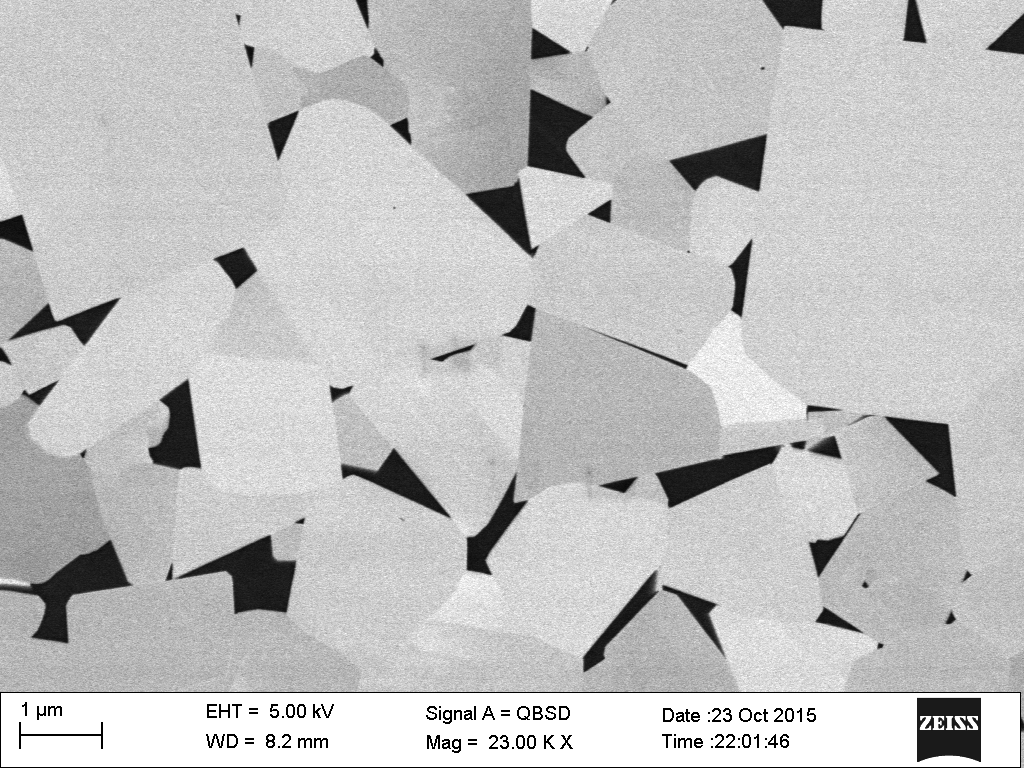
\includegraphics[width=0.5\linewidth]{wc_co_example}
\caption{Image of WC-Co hardmetal showing the characteristic WC grain shapes at 10\% Co by volume. Image courtesy of Amine Yousfi, Chalmers University of Technology.} \label{fig:wc-co_hardmetal}
\end{figure}

\begin{figure}[htbp!]
\centering
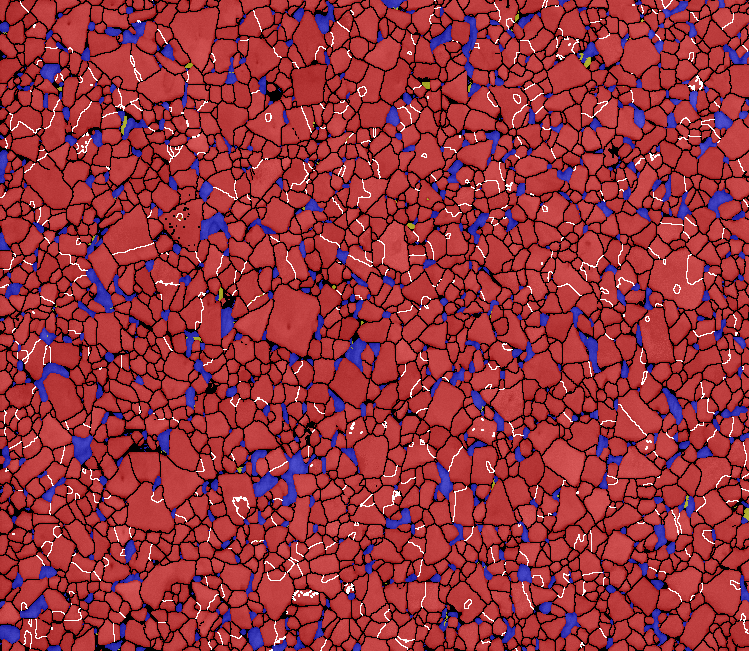
\includegraphics[width=0.5\linewidth]{wc-co-sigma2}
\caption{EBSD phase map with WC in red, Co in blue and $\Sigma$2 boundaries marked in white. Image courtesy of Mattias Elwing, Sandvik Tooling} \label{fig:sigma_2}
\end{figure}

WC-Co hardmetal consists primarily of WC grains in a Co matrix (volume fraction Co ranging between 5 to 30\%) with other trace elements that affect the grain shapes.
During manufacturing, a so called ``green-body'' of WC and Co powder is compressed and subsequently heated (so called liquid phase sintering).
Co acts as a binder, and by surface tension pulls the grains together creating (in ideal cases) a fully dense product.
During heating, the WC grain boundaries move considerably while Co accumulates at grain boundaries.
Some inter-grain boundaries have lower energy and may persist in the finished product, in the case of WC-Co systems the low energy $\Sigma$2-boundary (\SI{90}{\degree} misorientation) frequently occurs, as shown in Figure~\ref{fig:sigma_2}.

The finished product consists of interpenetrating WC and Co phases as shown in Figure~\ref{fig:wc-co_hardmetal}, and the WC grains hardness and wear resistance combined with the ductility of the Co binder phase leads to a material capable of working at high temperatures and at high loads, which makes the material suitable for cutting tools.

\begin{figure}[H]
  \centering
  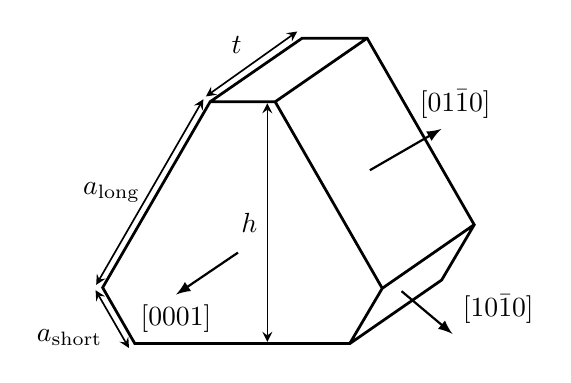
\begin{tikzpicture}[>=stealth,y=0.80pt, x=0.80pt, yscale=-0.4, xscale=0.4]
  \begin{scope}[shift={(-75.86158,-202.85562)}]
  \path[draw=black,line join=miter,line width=1.000pt]
    (279.5897,283.5098) -- (383.3845,211.7574)
    (400.3992,494.2529) -- (504.1964,422.3622)
    (206.1015,283.5760) -- (279.5851,283.5760) -- (400.4913,494.2006) -- (363.7495,556.5762) -- (121.0827,556.5762) -- (84.7681,493.3461) -- cycle
    (363.7472,556.6584) -- (467.6017,484.7860) -- (504.3435,422.4103) -- (383.4373,211.7858) -- (309.9537,211.7858) -- (206.0765,283.5226);

  \path[-latex,draw=black,line width=0.800pt] (386.5134,360.8340) -- (467.2742,314.2067) node[above] {\ \ \ $[01\bar{1}0]$};
  \path[-latex,draw=black,line width=0.800pt] (422.2673,497.3911) -- (479.8886,545.7595) node[above right] {$[10\bar10]$};
  \path[-latex,draw=black,line width=0.800pt] (237.5262,453.8704) -- (167.5691,501.2650) node[below] {$[0001]$};
  \path[<->,draw=black,line width=0.600pt]
    (270.7209,285.1513) -- (270.7209,554.6222) node[midway, left] {$h$};
  \path[<->,draw=black,line width=0.600pt]
    (198.4950,280.6057) -- (77.4371,490.2840) node[midway,left] {$a_{\text{long}}$};
  \path[<->,draw=black,line width=0.600pt]
    (76.7716,496.2732) -- (114.4794,561.5851) node[midway,below left] {$a_{\text{short}}$};
  \path[<->,draw=black,line width=0.600pt] (201.3188,277.5139) -- (304.4691,204.1695) node[midway,above left] {$t$};
  \end{scope}
  \end{tikzpicture}
  \caption{\label{fig:tt} The geometry of the truncated (equilateral) triangular prism from \cite{christensen_morphology_2007}.}
\end{figure}

The main microstructural parameters we aim to control in the synthetic microstructures are the volume fractions of WC and Co, $v_\text{WC}$ and $v_\text{Co}$, respectively ($v_\text{WC}+v_\text{Co}=1$), the grain shape and size distribution, and the contiguity.
The contiguity of the WC phase, $C$, is an important microstructural parameter as it relates grain boundary $A_\text{gb}$ and phase boundary $A_\text{pb}$ areas according to \cite{spiegler_finite_1992,lay_microstructure_2014}
\begin{equation}
	C = \frac{2 A_\text{gb}}{2 A_\text{gb} + A_\text{pb}}.
\end{equation}
The factor 2 is inserted in front of $A_\text{gb}$, since the contiguity is a measure of the degree of connection of one WC grain to other WC grains.
In addition to the volume fraction, the contiguity of the carbide phase is the most frequently documented microstructural parameter found in papers dealing with WC-Co hardmetals.

The morphology of WC grains has been analyzed in a series of papers \cite{christensen_quantitative_2005,christensen_morphology_2007,lay_morphology_2008}, and the truncated triangular prism has been identified as the equilibrium WC shape in a Co surrounding.
Its geometry is defined in e.g.\ \cite{christensen_morphology_2007}.
The WC grain shape is defined by the truncation factor
\begin{equation}
	r = \frac{a_\text{short}}{a_\text{long}}
\end{equation}
and the elongation factor
\begin{equation}
	k = \frac{t}{h}
\end{equation}
with $a_\text{short}$, $a_\text{long}$, $t$ and $h$ defined in Figure~\ref{fig:tt}.
The equilibrium $r$ and $k$ values depend on the carbon chemical potential, which in turn depends on temperature and alloy composition.
Experimental $r$ and $k$ values are reported in \cite{lay_morphology_2008}.
In order to look at size distributions, an equivalent sphere diameter, $d_\text{eq}$, is related to the volume of grain, $V$, by $\frac{\pi}{6} d_\text{eq}^3 = V$.
The parameters $r$, $k$ and $d_\text{eq}$ are assumed to be sufficient to fully define the shape and volume of a WC grain model..

%%%%%%%%%%%%%%%%%%%%%%%%%%%%%%%%%%%%%%%%%%%%%%%%%%%%%%%%%%%%%%%%%%%%%%%%%%%%%%%%%%%%%%%%%%%%%%%%%%%%%%%%%%%%%%%%%
%%%%%%%%%%%%%%%%%%%%%%%%%%%%%%%%%%%%%%%%%%%%%%%%%%%%%%%%%%%%%%%%%%%%%%%%%%%%%%%%%%%%%%%%%%%%%%%%%%%%%%%%%%%%%%%%%
%%%%%%%%%%%%%%%%%%%%%%%%%%%%%%%%%%%%%%%%%%%%%%%%%%%%%%%%%%%%%%%%%%%%%%%%%%%%%%%%%%%%%%%%%%%%%%%%%%%%%%%%%%%%%%%%%
\section{Modeling strategy} \label{sec:strategy}

%Due to the complex inter-grain surfaces of a densely grain structure, a voxel description was used instead of CAD/polygonal description.
A voxelized cubic domain of size $L$ is set up with total of number of voxels $M^3$.
The number of voxels is determined by a parameter $m$ which determines the number of voxels across the average grain size ($d_0$), such that $M = m \frac{L}{d_0}$.
Periodic boundary conditions are used to minimize boundary effects.
The WC grains are generated with given input distribution for $r$, $k$, and $d_\text{eq}$, which are assumed to be independent.
Orientations of the grains are uniformly sampled, however, the packing strategy (discussed in Section~\ref{sec:grain_placement}) determines the positions used for the midpoint of each grain.
Some overlapping regions of WC-grains is present after insertion, and this is discussed in Section~\ref{sec:overlapping_grains}.

\subsection{Volume fraction control} \label{sec:volume_fraction_control}

The primary user input for CCBuilder is the volume fraction WC, $v_\WC$, or equivalently Co, $v_\Co = 1 - v_\WC$.
We note that the volume fraction $v_\WC$ is an average property which should hold true for averaging many realizations or as $L \to \infty$.
Just as small ``window'' of the real microstructure may have a higher or lower $v_\WC$ present, this effect is obtained in CCBuilder as well.
In order to keep the microstructure properties independent of chosen domain size $L$ and discretization $m$, a set of grains is generated targeting a volume fraction, $v_{\WC,\text{goal}}$, that does not account for the (unknown) overlap.
%
% This is due to  though only on average, as any given ``window'' of the microstructure may have more or less actual volume fraction WC.
%
However, targeting the actual (final) average volume fraction, $v_\WC$, is very important.
Therefore the relation between $v_\WC$ and $v_{\WC,\text{goal}}$ is investigated in Figure~\ref{fig:sens_vol}, with the curve fit given in \eqref{eq:v_wc}.
Using \eqref{eq:inverse_v_wc} the actual (average) volume fraction can be controlled.
%These idealized grain shapes are not preserved in the packing stage, as some details are lost where grains contact.
% Post-processing is done with a Monte-Carlo simulation of a Potts model where grain boundaries are minimized in the overlapping regions.
%This creates more realistic grain shapes and further lowers the contiguity.
% Due to the potential in \eqref{eq:potential} and the grain sorting in the packing strategy, a complete list of grains need to be generated before insertion.


\subsection{Placement of WC grains} \label{sec:grain_placement}

\begin{figure}[H]
 \centering
  \begin{subfigure}[b]{0.23\linewidth}
  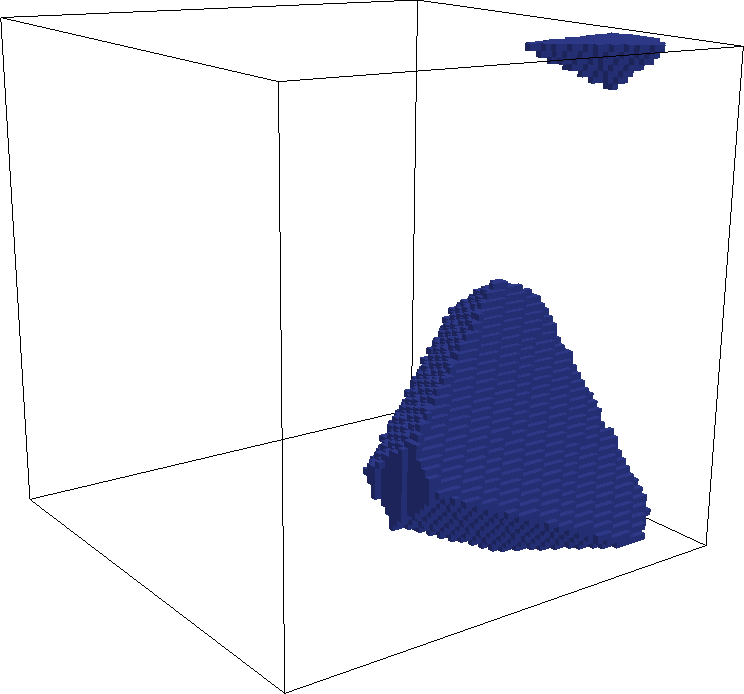
\includegraphics[width=1\linewidth]{step1}
  \caption{1 grain}
  \end{subfigure}
  \quad
  \begin{subfigure}[b]{0.23\linewidth}
  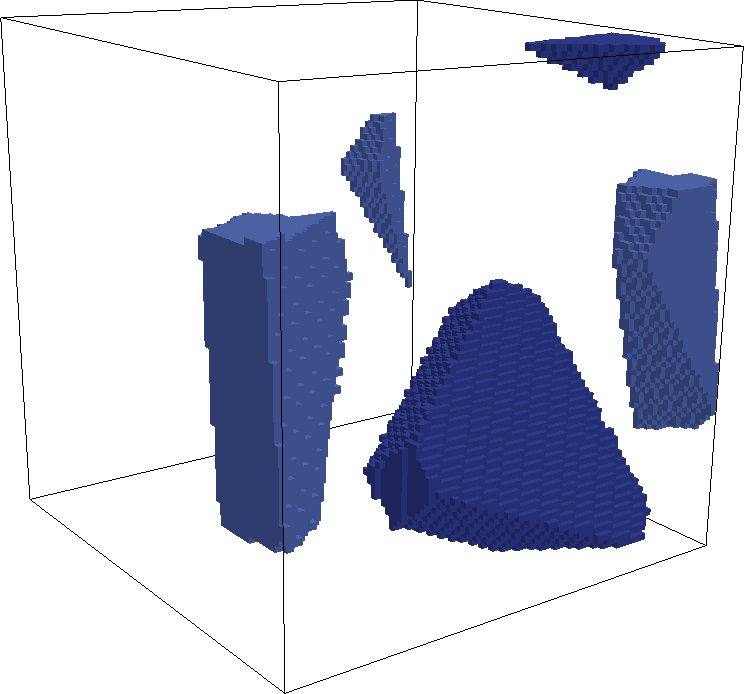
\includegraphics[width=1\linewidth]{step2}
  \caption{2 grains}
  \end{subfigure}
\\
  \begin{subfigure}[b]{0.23\linewidth}
  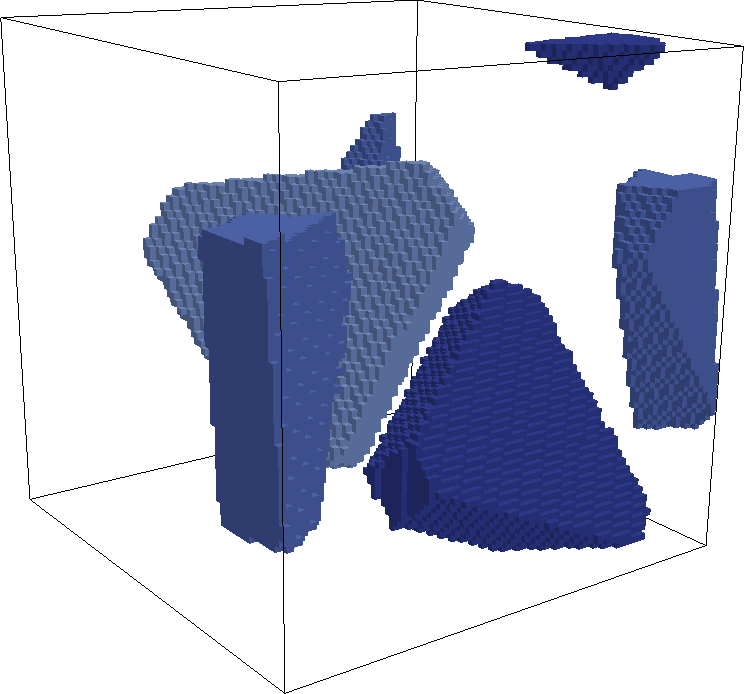
\includegraphics[width=1\linewidth]{step3}
  \caption{3 grains}
  \end{subfigure}
  \quad
  \begin{subfigure}[b]{0.23\linewidth}
  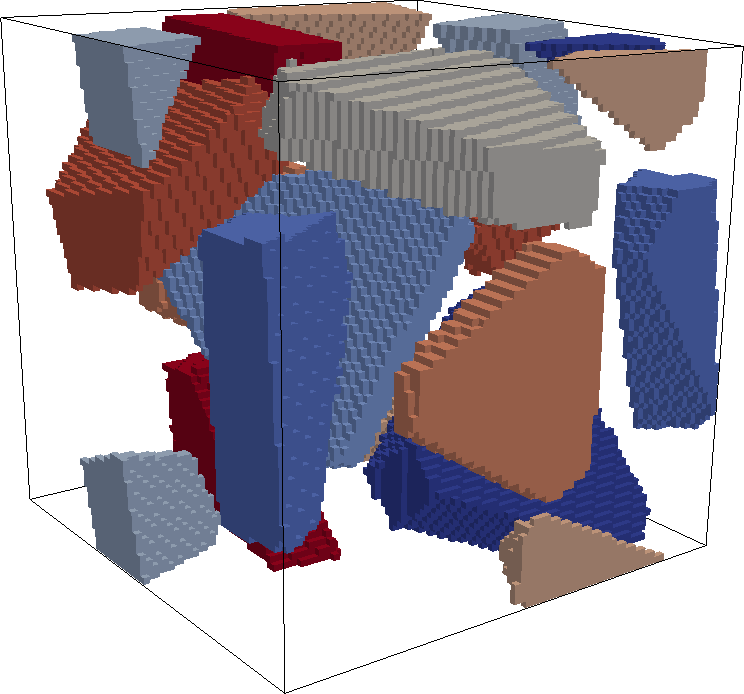
\includegraphics[width=1\linewidth]{step10}
  \caption{10 grains}
  \end{subfigure}

  \caption{\label{fig:ccbuilder_steps} Step by step of the first grains inserted into the voxel domain, showing the periodic boundaries}
\end{figure}

Several strategies for inserting the grains are implemented in order to obtain realistic microstructures. 
The generated grains are inserted one by one into the voxel domain, as illustrated in Figure~\ref{fig:ccbuilder_steps}.
When a voxel is already occupied by a different grain, the voxel is marked as an overlapping region.
These overlapping regions are dealt with in the final stage of the analysis.
The placement strategies are as follows:
%
\begin{itemize}
 \item \emph{Random placement}: A random position inside the domain is used for every grain independently.

 \item \emph{Repulsive potential}:
 Packing of the grains are performed by minimization of the potential $U$ defined as
\begin{equation}
  U = \sum_{i,j,i\neq j} \begin{cases}
	(V_i + V_j) (\left| \vec{r}_{ij} \right| - r_{0,ij})^2 / r_{0,ij}^2 & \text{if } \left|\vec{r}_{ij}\right| < r_{0,ij}
	\\
	0 & \text{otherwise}
      \end{cases}
  \label{eq:potential}
\end{equation}
 where $\vec{r}_{ij}$ is the vector between grain center $i$ and $j$, $V_i$ and $V_j$ are the respective grain volumes, and $r_{0,ij} = \frac12(d_{\text{eq},i}+d_{\text{eq},i})$, i.e.\ the sum of each grains equivalent radius.
 Only a local minimization using random initial grain positions is considered.
 
 \item \emph{Multiple random translations}:
 Using a brute-force method grains are randomly translating the grains within a given distance, $\Delta$, from either the random or optimized initial position.
 The random translation that yielded smallest overlap is then used.
 If random placement is allowed over the entire domain size, $\Delta = L/2$, the pre-optimized positions are of course no longer needed as the starting points.

\end{itemize}
It is important to note that during the grain placement the grain orientations are held fixed for all grains, as not to induce and unwanted artificial anisotropy.
The effect of a high packing factor is visualized in Figure~\ref{fig:random_vs_packing} where roughly twice as many grains were needed to be inserted to reach the same volume fraction as the one with packing enabled.
Comparing with Figure~\ref{fig:random_vs_packing} with Figure~\ref{fig:wc-co_hardmetal} we see that the high packing factor produces a visually more realistic grain structure.


With computational time that scale with the number of voxels, $M^3$, the grain placement with random translations can take considerable computational time.
Using a coarse grid the computational time can be sped up significantly.
This coarse grid isn't desirable in the final output, so using the new grain positions obtained from the coarse grid, the grains can then be reinserted into a fine grid without any additional packing.
% The minimum resolution required of the coarse grid is determined by the size of the WC-grains, but $5\si{\per\micro\meter} L \leq M_\text{coarse} \leq 10\si{\per\micro\meter}L$ is sufficient to capture the  grain shape for the size distribution used in this paper.

%%%%%%%%%%%%%%%%%%%%%%%%%%%%%%%%%%%%%%%%%%%%%%%%%%%%%%%%%%%%%%%%%%%%%%%%%%%%%%%%%%%%%%%%%%%%%%%%%%%
\subsection{Overlapping grains}\label{sec:overlapping_grains}

After placement, grains may overlap where the voxel belongs to 2 or more grains.
This has to be corrected for, and we handle the overlap by searching for a resulting grain boundary with low grain boundary area.
In principle, the ground boundary energy should be the minimized quantity, cf.\ Wahnström et. al \cite{????_wahnstrom_20??}, which would be possible using the available grain orientations.
However, in the present case, the ground boundary energy is simplified to the case of isotropic and homogeneous surface energy where minimization of area is equivalent.

Initially, each voxel in overlap is set to the first grain to have been placed there, creating a ground boundary area $A_0$.
We denote the minimum by $A_\text{min}$ and use a Monte Carlo procedure to search for a configuration with a grain boundary area $A_n$ given by the probability
\begin{align}
 P_n \propto e^{-\frac{A_n - A_\text{min}}{\tau}}
\end{align}
i.e.\ we allow $\dif A = A_n - A_\text{min}$ from the minimum value with a probability proportional to $e^{-\dif A / \tau}$.
Here $\tau$ is a control parameter with dimension of area.
Since a voxel in overlapping regions can belong to several grains, out model can be viewed as a Potts model.

To change from configuration $m$ to configuration $n$ a voxel is randomly chosen from the overlapping regions and it is checked whether it is at a grain boundary.
If so, the voxel is randomly changed to one of the neighboring WC grains, and we compute the difference in total grain boundary area, $\dif A_{nm} = A_n - A_m$.
To fulfill detailed balance we use the standard Metropolis recipe, i.e.\ if $\dif A_{nm} \leq 0$ the change is accepted with unit probability, otherwise with probability $e^{-\dif A_{nm}/\tau}$.
The area $\dif A_{nm}$ is measured in the number of voxel boundaries, ranging from -6 to 6 and an appropriate value for $\tau$ is $0.5$, which gives a \SI{13.5}{\percent} probability to increase the area by one.

A problem with the present procedure is the simplified approximation of the area, which is tied to the exact voxel description through the 6 neighboring voxels.
This means that rotating the domain window would produce a significantly different microstructure.


% After placing the grains, it is possible to run a Potts model simulation \cite{holm_computer_2001} of the structure to correct the overlapping regions, minimizing the grain boundary area, $A_\text{gb}$.
% The effect of the simulation is illustrated in Figure~\ref{fig:potts_before_after}, which shows that all the grains obtain more convex shape after the Potts simulation, which is closer to real microstructures, see Figure~\ref{fig:wc-co_hardmetal}.
% %
% The simulation uses the Metropolis algorithm in analogy with typical Ising model simulations.
% In the Potts algorithm, a voxel is randomly chosen from the overlapping regions and it is checked whether it is at a grain boundary.
% If so, the integers of the neighboring voxels that are different from the chosen voxel are inserted into a set, i.e.\ each of the integers of the neighboring grains occurs only once in the set.
% The voxel is randomly changed to one of the neighboring WC grains, the difference in total grain boundary area, $\text{d}A$, due to the change is computed.
% % Then an integer is chosen at random from this set and the chosen voxel assigned with this integer.
% If $\text{d}A \leq 0$ the change is accepted.
% If $\text{d}A > 0$ the change is accepted with a (small) probability $\exp(-\text{d}A / \tau)$, where $\tau$ is a fictitious material parameter.
% It should be noted that $\tau$ does not correspond to a physical parameter, as the voxels are several order of magnitude larger than individual atoms.

For performance, a multi-grid approach is used for the Potts model simulation as well.
The simulation first run on a coarser resolution, $m_\text{coarse} = \frac12 m$, with identical grain placement.
The results are then projected over from the coarse grid to the fine grid in the regions with overlap.
It is necessary to run an additional Potts model simulation on the fine grid to clear out the artefacts left from the coarse grid, however, much fewer steps are required in total.


%%%%%%%%%%%%%%%%%%%%%%%%%%%%%%%%%%%%%%%%%%%%%%%%%%%%%%%%%%%%%%%%%%%%%%%%%%%%%%%%%%%%%%%%%%%%%%%%%%%
%%%%%%%%%%%%%%%%%%%%%%%%%%%%%%%%%%%%%%%%%%%%%%%%%%%%%%%%%%%%%%%%%%%%%%%%%%%%%%%%%%%%%%%%%%%%%%%%%%%
%%%%%%%%%%%%%%%%%%%%%%%%%%%%%%%%%%%%%%%%%%%%%%%%%%%%%%%%%%%%%%%%%%%%%%%%%%%%%%%%%%%%%%%%%%%%%%%%%%%
\section{CCBuilder} \label{sec:ccbuilder}

\begin{figure}[H]
  \centering
  \begin{tabular}{l|l}
   \toprule
   Parameter & Description
   \\ \midrule
   $L$ & Domain size
   \\
   $k$, $r$, $d_\text{eq}$ & Grain geometry (given as distributions)
   \\
   $v_{\WC,\text{goal}}$ & Target volume fraction (not accounting for overlap)
   \\ \midrule
   $m$ & Average number of voxels across each grain (grid resolution)
   \\
   $\text{MC}_\text{steps}$ & Controls the number of Monte-Carlo steps for the Potts model simulation
   \\
   $N_\text{tries}$ & Number of random translations during packing
   \\
   $\Delta$ & Distance for allowed random translations during packing (set to $L/2$ by default)
   \\
   \bottomrule
  \end{tabular}
  \caption{\label{tab:input_data} Input parameters (physical parameters on top) for running CCBuilder.}
\end{figure}

The modeling strategy described in Section \ref{sec:strategy} has been implemented in a new software named CCBuilder (Cemented Carbide Builder).
For simplicity, CCBuilder is mainly written in Python with computationally extensive functions implemented in Cython (\url{http://cython.org}), which is a superset of the Python language which adds static type declarations.
This allows automatic conversion of Cython code into C code, which can be compiled and optimized to native binaries.
If the Cython code is carefully written, i.e.\ all variables are typed, contents of arrays are accessed through C pointers, bounds checks are disabled etc., the produced binaries have performance fully on par with ``hand-written'' C code.
Source code and future developments of CCBuilder is available on GitHub (\url{https://github.com/Micket/CCBuilder}).
The main entry point of the software is a control script named \verb+make_cc.py+ which comes with suitable parameters predefined.
The list of input parameters are listed Table~\ref{tab:input_data}.
The control script is setup to target specific goals what steps to perform.


% To allow full control of the microstructure generation, it was decided to write new separate code, named CCBuilder, for the WC-Co structure using the same kind of voxel representation as in Dream3D.
% Dream3D is a promising piece of software as it includes e.g.\ functionality for surface meshing.
% Therefore, the output data structure of CCBuilder is made fully compatible with Dream3D data files to allow importing data into Dream3D for further processing.

In CCBuilder, a list of prisms is generated by the function \verb|prepare_triangles| based on the truncated prism as defined in Figure~\ref{fig:tt}.
The inputs are the distributions for $r$, $k$, $d_\text{eq}$, and the target volume fraction $v_{\WC,\text{goal}}$.
The control script comes predefined with uniform distributions for the grain shape and size; $r \in U[r_\text{min},r_\text{max}]$ and $k \in U[k_\text{min},k_\text{max}]$, $d_\text{eq} \in U[d_\text{eq,min},d_\text{eq,max}]$.
The average grain size $d_0$ defines the length scale.
%
To each grain, there is an associated rotation matrix, which defines the rotation state of the grain with respect to the $\hat{x}, \hat{y}, \hat{z}$ directions of the volume.
The rotation matrix is drawn from a distribution of uniformly random rigid rotations using the algorithm of Brannon \cite{brannon_rotation:_2002}.
The number of generated prisms is controlled by a goal WC volume fraction $v_{\WC,\text{goal}}$ and new grains are generated until $\sum_j V_j > v_{\WC,\text{goal}}L^3$, i.e.\ a volume fraction that does not take into account the overlap between WC grains.
% An initial midpoint of each prism is drawn from a uniform distribution $[0,L]^3$.
The grains obtain a random position within the domain, and the function \verb+optimize_midpoints+ can be used to separate the grains (before any discretization is introduced) by minimizing the potential in \eqref{eq:potential}.


In the function \verb|populate_voxels|, the actual grain placement and assignment of voxels takes place.
In CCBuilder, the volume considered is a cube of side $L$ divided into $M$ divisions giving a total of $M^3$ voxels represented in an integer array.
%
Each voxel is assigned an integer $i$ representing the binder or the WC grain to which it belongs, where $i=1$ means Co binder and $i = 2, 3, \ldots$ means that the voxel belongs to WC grain number $i-2$ (numbered from $0$).
The algorithm starts by initializing the volume as a pure binder, i.e.\ all ones.
The WC grains are then one by one inserted into the voxel structure.
For each grain a list of voxel indices is prepared by the function \verb|make_voxel_indices|.
The generated lists contain the voxels lying inside each grain and is made under periodic boundary conditions to eliminate any boundary effects.
%
The algorithm takes the first prism and assigns the voxels lying inside it and for each subsequent prism a number of tries with random translation is made to insert the prism, as can be seen in Figure~\ref{fig:ccbuilder_steps}, where we can see that the first few grains manage to avoid any overlap.
% % After the $N_\text{tries}$ tries within the user defined distance $\Delta$, the position with minimum overlap with the existing grains is chosen.
After the $N_\text{tries}$ tries the position with minimum overlap with the existing grains is chosen.

%%%%%%%%%%%%%%%%%%%%%%%%%%%%%%%%%%%%%%%%%%%%%% POTTS:

The Potts model simulation is implemented as described in Section~\ref{sec:strategy} in the function \verb|make_mcp_bound|.
% The change in total area, $\text{d}A$, is computed by checking each neighboring voxel.
After laying out the WC grains as described earlier, all WC/Co interfaces are of either $\text{WC}\{0001\}/\text{Co}$ or $\text{WC}\{10\bar{1}0\}/\text{Co}$ orientation, which is reasonable given the strong tendency of WC to facet along these surfaces when sintered in Co \cite{kim_interface_2008}.
The grains are therefor limited in extent to their original truncated triangular prism shapes as determined in the initial run of the function \verb|prepare_triangles|.
This limits grain boundary movement and maintains the $\text{WC}\{0001\}/\text{Co}$ or $\text{WC}\{10\bar{1}0\}/\text{Co}$ orientations of most phase boundaries, while still allowing unphysical artefacts in the overlapping regions to ``heal''.
% \color{red} \textbf{UNFINISHED!!!!! Not sure what Sven means with some of this?}
% In \verb|make_mcp_unlim|, there is no limit to the growth of individual grains and, hence, considerable movement of grain boundaries is likely to take place during the simulation.
% This is probably unwanted, as it leads to changes in WC morphology.
% 
% After a Potts simulation run, the prism shape of some WC grains will have changed considerably as larger grains have ``invaded'' initially small grains, and WC/Co interfaces will as a result be more randomly distributed.
% In \verb|make_mcp_bound|, the grains are limited in extent to their original truncated triangular prism shapes as determined in the initial run of the function \verb|prepare_triangles|.
% This limits grain boundary movement and maintains the $\text{WC}\{0001\}/\text{Co}$ or $\text{WC}\{10\bar{1}0\}/\text{Co}$ orientations of most phase boundaries, while still allowing unphysical artefacts to ``heal''.
% \color{black}

The function \verb|write_hdf5| writes the simulation to an HDF5 file (\url{http://www.h5py.org}), which can be analyzed further in the microstructure analysis software Dream3D (\url{http://dream3d.bluequartz.net}) and in Paraview (\url{http://www.paraview.org}).


\subsection{Analysis tools} \label{sec:analysis_tools}

In order to determine the statistical properties of the microstructure, a number of post-processing tools where developed to analyze the finished voxel representation.
\begin{itemize}
 \item Bulk properties such as Euler angles of the WC grain orientation, total phase volumes, and grain volumes are calculated with \verb+calc_grain_prop+.
 \item Surface properties such as surface voxels (WC-WC and WC-Co), grain boundary voxels (WC-WC), and interface voxels (WC-Co) are computed with \verb+calc_surface_prop+.
 \item The Co grain sizes are computed with \verb+compute_co_grain_sizes+. Co grain size is used to determine the connectivity of the Co matrix.
 \item Equivalent diameter of the final grain volumes are calculated with the function \verb+volume_to_eq_d+.
 \item The misorientations of all contacting WC grain-pairs is computed by the function \\ \verb+compute_all_misorientation_voxel+, taking into account the trigonal symmetries of the WC grains.
%  \item Mass fractions can be obtained through the simple function \verb+mass_fraction+ for convenience.
\end{itemize}
Many of bulk and surface properties are exported in the HDF5 format using the function \verb+write_hdf5+, which can be visualized and analyzed in Paraview and Dream3D.
All these tools are called by the control script.


%%%%%%%%%%%%%%%%%%%%%%%%%%%%%%%%%%%%%%%%%%%%%%%%%%%%%%%%%%%%%%%%%%%%%%%%%%%%%%%%%%%%%%%%%%%%%%%%%%%
%%%%%%%%%%%%%%%%%%%%%%%%%%%%%%%%%%%%%%%%%%%%%%%%%%%%%%%%%%%%%%%%%%%%%%%%%%%%%%%%%%%%%%%%%%%%%%%%%%%
%%%%%%%%%%%%%%%%%%%%%%%%%%%%%%%%%%%%%%%%%%%%%%%%%%%%%%%%%%%%%%%%%%%%%%%%%%%%%%%%%%%%%%%%%%%%%%%%%%%
\section{Results and discussion}
\label{sec:results}

The average size of grain in WC-Co system varies by several magnitudes depending on the application.
For this purpose, we define a length scale parameter $d_0$ to represent the average grain size.
In the examples shown in this paper we choose $d_0 = \SI{1}{\micro\meter}$, with the corresponding size distribution $d_\text{eq} \in U[0.5, 1.5]$ \cite{lay_morphology_2008}.
Some variations of the of the size distribution is investigated in Section~\ref{sec:grain_size_dist}.
Using $d_0$ we can obtain the approximate number of grains, $N$, in the final microstructure 
\begin{align}
 &\nonumber \frac{4\pi}{3} \left(\frac{d_0}{2}\right)^2 N = v_\WC L^3 \implies 
 \\
 &N = 2 v_\WC \left(\frac{L}{d_0}\right)^3 \approx 2 v_{\WC,\text{goal}} \left(\frac{L}{d_0}\right)^3 \propto \left(\frac{L}{d_0}\right)^3
\end{align}
which lets us pick a reasonable domain size $L$ based on the desired number of grains.
The lengths $d_0$ and $L$ can be scaled arbitrarily to match any real WC-Co system.

The grain shape distributions are chosen as $r \in U[0.1, 0.4]$, $k \in U[0.4, 1.4]$, which are typical values for high $W$ content.
The comparison to experimental value also include flatter grains, $k \in U[0.1, 0.4]$, which are typical for high $C$ content, cf. \cite{lay_morphology_2008}, which has a significant effect on the packing using the repulsive potential.


The discretization parameter $m$ is chosen according to the desired number of voxels across the average grain.
This parameter should at least be set to $m = 10$ in order to obtain recognizable grain shapes after discretization.
The resulting number of voxels along each coordinate axis is obtained as $M = m \frac{L}{d_0}$.

The volume fraction is indirectly controlled through the target volume fraction not accounting for overlap, $v_{\WC,\text{goal}}$.
For the most results we use $v_{\WC,\text{goal}} = 1.0$ which gives a moderate final volume fraction of $v_\WC \approx 0.87$ for the highest packing factor.



\subsection{Packing strategy}
\begin{figure}[H]
  \centering
  %
  \begin{tikzpicture}[font=\footnotesize]
  \begin{axis}[
      xmax = 2.0,
      xmin = 0.,
      ymin = 0.0,
      ymax = 1.0,
      legend pos=south east,
      legend style={font=\tiny},
      legend style={draw=none},
      xlabel={$v_{\WC,\text{goal}}$},
      ylabel={$v_\WC$},
      width=0.45\linewidth
      ]

    \addplot[red, error bars/.cd, y dir=both, y explicit]
	table[x=target_frac, y expr=1-\thisrow{co_fracs_mean}, y error expr=\thisrow{co_fracs_std}] {stat_vol_random_L10.0.txt};
    \addlegendentry{Random placement}

    \addplot[green!50!black, error bars/.cd, y dir=both, y explicit]
	table[x=target_frac, y expr=1-\thisrow{co_fracs_mean}, y error expr=\thisrow{co_fracs_std}] {stat_vol_U_L10.0.txt};
    \addlegendentry{Repulsive potential}
    
    \addplot[blue, error bars/.cd, y dir=both, y explicit]
	table[x=target_frac, y expr=1-\thisrow{co_fracs_mean}, y error expr=\thisrow{co_fracs_std}] {stat_vol_transl_L10.0.txt};
    \addlegendentry{Random translations}
  \end{axis}
  \end{tikzpicture}
  %
  \begin{tikzpicture}[font=\footnotesize]
  \begin{axis}[
      xmax = 2,
      xmin = 0.,
%       ymin = 0.0,
%       ymax = 1.0,
      legend pos=south west,
      legend style={font=\tiny},
      legend style={draw=none},
      xlabel={$v_{\WC,\text{goal}}$},
      ylabel={$\mathop{\text{mean}}(d_{\text{eq}})$},
      width=0.45\linewidth
      ]

    \addplot[red, error bars/.cd, y dir=both, y explicit]
	table[x=target_frac, y=d_eq_mean_mean, y error expr=\thisrow{d_eq_mean_std}] {stat_vol_random_L10.0.txt};
    \addlegendentry{Random placement}

    \addplot[green!50!black, error bars/.cd, y dir=both, y explicit]
	table[x=target_frac, y=d_eq_mean_mean, y error expr=\thisrow{d_eq_mean_std}] {stat_vol_U_L10.0.txt};
    \addlegendentry{Repulsive potential}
    
    \addplot[blue, error bars/.cd, y dir=both, y explicit]
	table[x=target_frac, y=d_eq_mean_mean, y error expr=\thisrow{d_eq_mean_std}] {stat_vol_transl_L10.0.txt};
    \addlegendentry{Random translations}
  \end{axis}
  \end{tikzpicture}
%   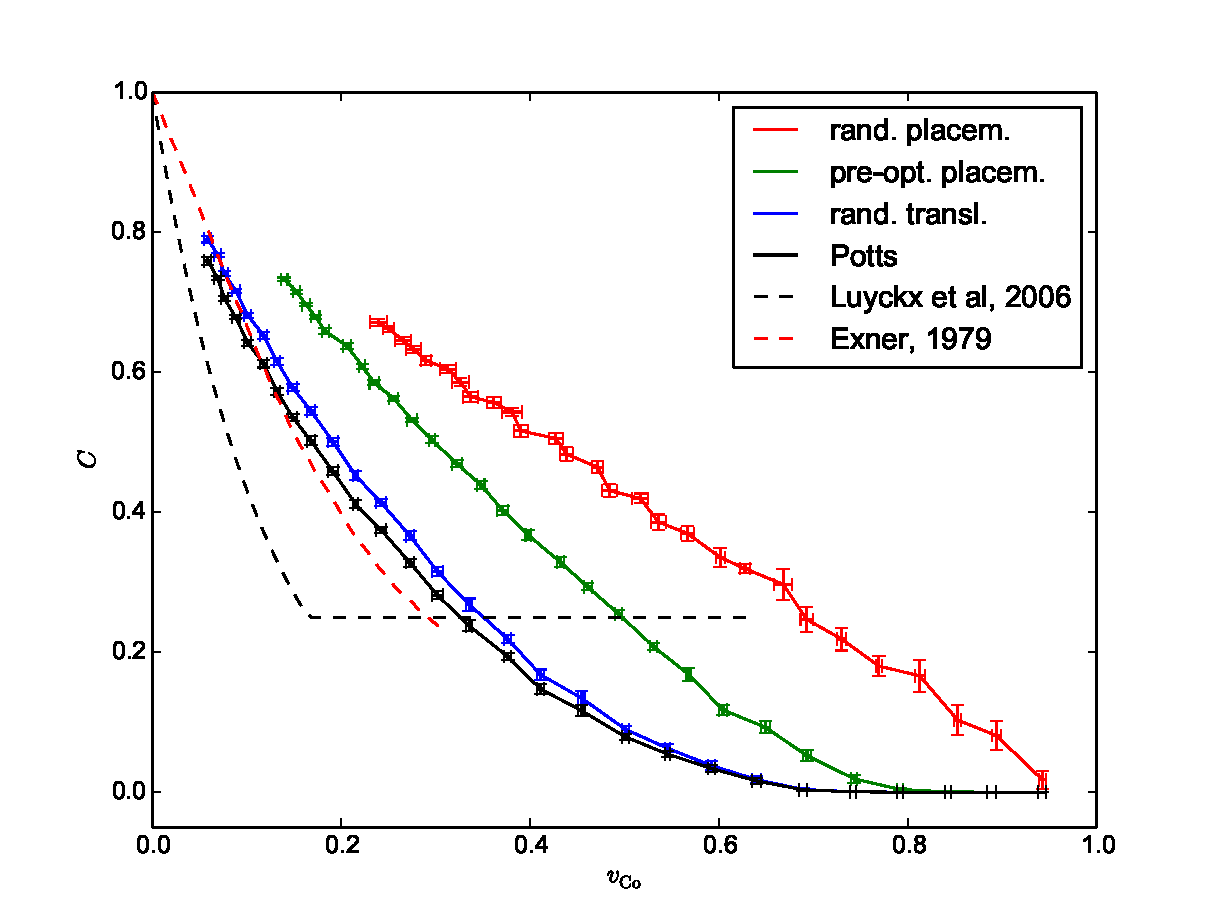
\includegraphics[width=0.6\linewidth]{Result_plots/runs1/contiguity}
  \caption{Comparison of packing strategies. Bars indicate one standard deviation.}
  \label{fig:sens_vol}
\end{figure}

\begin{figure}[H]
 \centering
  \includegraphics[width=.15\linewidth]{IPF}
  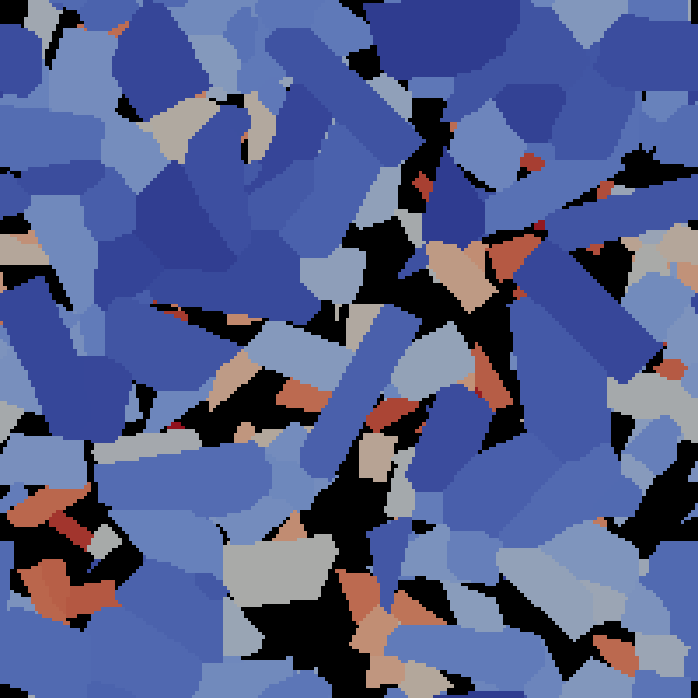
\includegraphics[width=0.3\linewidth]{ccbuilder_random_cs}
  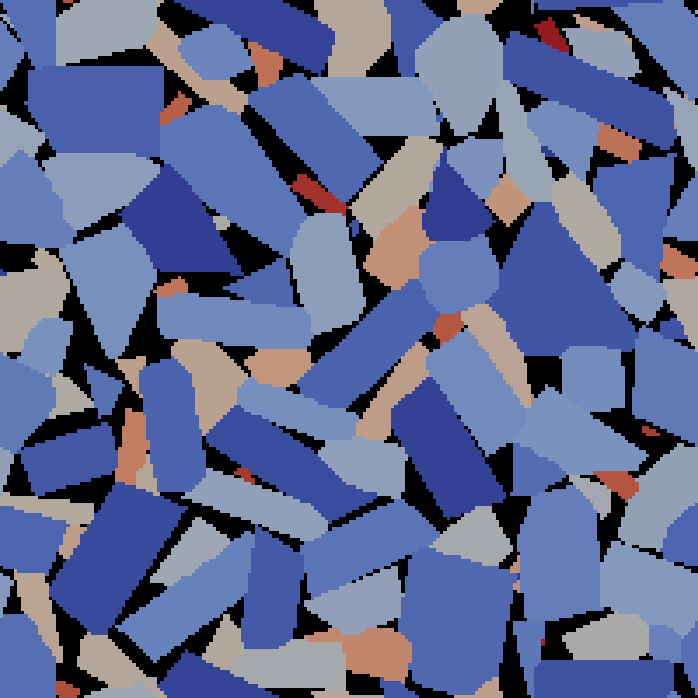
\includegraphics[width=0.3\linewidth]{ccbuilder_packed_cs}
  % 0.859249
  \caption{\label{fig:random_vs_packing} Cross-section of CCBuilder output with randomly placed grains (left) and with packed grains (right) with equal volume fraction Co, $v_\Co$}
\end{figure}


In Figure~\ref{fig:sens_vol} results are obtained for 5 realizations using $L=\SI{10}{\micro\meter}$, $m=10$.
The visual effect of a high packing factor using the random translations is shown in Figure~\ref{fig:random_vs_packing}.
The random positions are used as the start point for the repulsive potential, which is a local minimization.
The random translations used $N_\text{tries} = 2500$ with $\Delta = L/2$ (movement over entire domain), which yields a high packing factor.

% As grain size distribution is not always documented in articles, the best option for comparing the grain structure morphology is the contiguity.
% In Figure~\ref{fig:contiguity_grain_size} we see three different grain placement strategies compared with experimental results.
% With the random grain placement, reaching the lower $v_\Co$ is not possible without generating unrealistic grain shapes due to excessive overlap, and as a result, the contiguity is far off the experimental results.
% The result show an excellent agreement with Exners curve  \cite{exner_physical_1979}, but a different trend is see in data by Luyckx \cite{luyckx_dependence_2006}.
% However, with the packing strategy discussed in Section~\ref{sec:method} we obtain results within the span of the experimental measurements, and the Potts simulation further improves this.


Using the results in Figure~\ref{fig:sens_vol} we can fit a curve to match correlate the input parameter $v_{\WC,\text{goal}}$ to the obtained value $v_\WC$ in order to control the parameter more easily.
When using random translations, the trend is linear from zero to $v_\WC = \frac12$, up to which packing is typically achieved with no overlap.
After this, $v_\WC$ asymptotically approaches 1 as $v_{\WC,\text{goal}}$ approaches infinity.
With this in mind, the following function is adopted for curve-fitting
\begin{align}
 v_\WC &= \begin{cases}
  1 - \frac12\exp(- 2(v_{\WC,\text{goal}} -\frac12) - \alpha(v_{\WC,\text{goal}} -\frac12)^2 ), & v_{\WC,\text{goal}} \geq \frac12
  \\
  v_{\WC,\text{goal}}, & v_{\WC,\text{goal}} \leq \frac12
 \end{cases}
 \label{eq:v_wc}
 \\ 
 &\implies\nonumber
 \\
 v_{\WC,\text{goal}} &= \begin{cases}
    \frac{\alpha - 2}{2\alpha} + \frac1\alpha \sqrt{1 - \alpha\log(-2(v_\WC-1))} & v_\WC \geq \frac12
    \\
    v_\WC & v_\WC \leq \frac12
                       \end{cases}
                       \label{eq:inverse_v_wc}
\end{align}
where $\alpha = 1.3$ gives a perfect fit with the random translation results in Figure~\ref{fig:sens_vol}.
Changing any of the shape and size distributions or the packing strategy will affect the obtained volume fraction. 


\subsection{Potts model simulation}

\begin{figure}[H]
  \centering
  \includegraphics[width=.15\linewidth]{IPF}
  \includegraphics[width=.3\linewidth]{ccbuilder_packed_nopotts}
  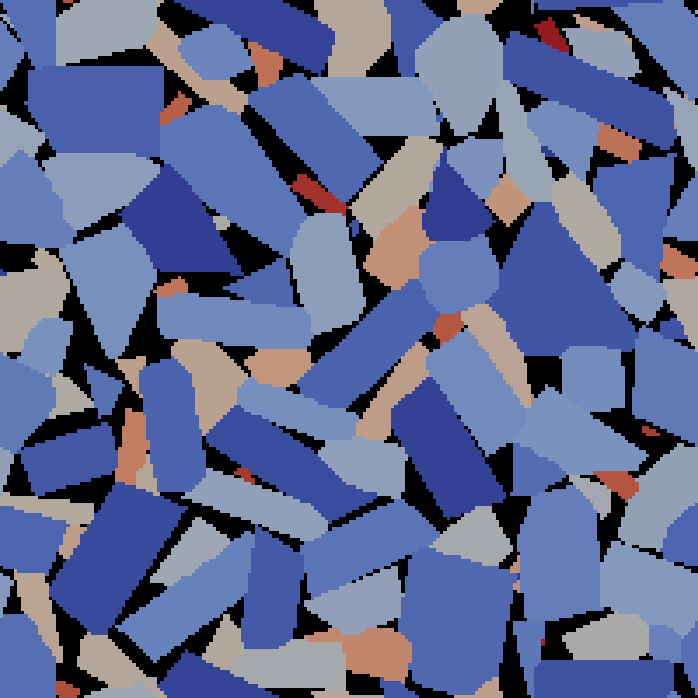
\includegraphics[width=.3\linewidth]{ccbuilder_packed_cs}
  \caption{\label{fig:potts_before_after} A slice of a generated microstructure before (left) and after (right) Potts model simulation with grain boundaries highlighted. Binder is shown in black.}
\end{figure}

\begin{figure}[H]
  \centering

  \begin{tikzpicture}[font=\footnotesize]
  \begin{axis}[
      xmax = 1,
      xmin = 0.,
      ymin = 0.0,
      ymax = 1.0,
      legend pos=north east,
      legend style={font=\tiny},
      legend style={draw=none},
      xlabel={$v_\Co$},
      ylabel={$C$},
      width=0.45\linewidth
      ]
%     \addplot[mark=x, only marks,forget plot] table[x index=8,y index=3]  {luyckx_table.txt};
    %\addlegendentry{Ultra fine}
%     \addplot[mark=x, only marks,forget plot] table[x index=8,y index=7]  {luyckx_table.txt};
    %\addlegendentry{Fine}
%     \addplot[mark=x, only marks,forget plot] table[x index=8,y index=12]  {luyckx_table.txt};
    %\addlegendentry{Medium}
%     \addplot[mark=x, only marks] table[x index=8,y index=16]  {luyckx_table.txt};
    %\addlegendentry{Coarse}
%     \addlegendentry{Luyckx et al.\ (2006)}
%     \addplot[mark=*, only marks] coordinates { (0.15, 0.42) };
%     \addlegendentry{Chang et al.\ (2015)}
    
%     \addplot[black, dashed] table[x index=0,y index=1]  {exner_table.txt};
%     \addlegendentry{Exner (1979)}

    \addplot[red, error bars/.cd, y dir=both, y explicit]
	table[x=co_fracs_mean, y=cont_mean, y error expr=\thisrow{cont_potts_std}] {stat_vol_random_L10.0.txt};
    \addlegendentry{Random placement}

    \addplot[green!50!black, error bars/.cd, y dir=both, y explicit]
	table[x=co_fracs_mean, y=cont_mean, y error expr=\thisrow{cont_potts_std}] {stat_vol_U_L10.0.txt};
    \addlegendentry{Repulsive potential}
    
    \addplot[blue, error bars/.cd, y dir=both, y explicit]
	table[x=co_fracs_mean, y=cont_mean, y error expr=\thisrow{cont_potts_std}] {stat_vol_transl_L10.0.txt};
    \addlegendentry{Random translations}
    
    
    \addplot[red, dashed, error bars/.cd, y dir=both, y explicit]
	table[x=co_fracs_mean, y=cont_potts_mean] {stat_vol_random_L10.0.txt};
%     \addlegendentry{Random placement}

    \addplot[green!50!black, dashed, error bars/.cd, y dir=both, y explicit]
	table[x=co_fracs_mean, y=cont_potts_mean] {stat_vol_U_L10.0.txt};
%     \addlegendentry{Repulsive potential}
    
    \addplot[blue, dashed, error bars/.cd, y dir=both, y explicit]
	table[x=co_fracs_mean, y=cont_potts_mean] {stat_vol_transl_L10.0.txt};
%     \addlegendentry{Random translations}
  \end{axis}
  \end{tikzpicture}
  \caption{Comparison of packing strategies. Dashed lines indicate values after Potts model simulation. Bars indicate one standard deviation.}
  \label{fig:sens_vol2}
\end{figure}

The primary reason for the introduction of a Potts model simulation after packing is to reduce the number of unrealistic grain shapes in overlapping regions, as shown in Figure~\ref{fig:potts_before_after}.
As the grain boundary area is minimized, one can also see a drop in contiguity around $0.02$ -- $0.05$, as shown in Figure~\ref{fig:sens_vol2}, depending on the grain placement.




\subsection{Sensitivity to voxel density}
%%%%%%%%%%%%%%%%%%%%%%%%%%%%%%%%%%%%%%%%%%%%%%%%
%%%%%%%%%%%%%%%%%%%%%%%%%%%%%%%%%%%%%%%%%%%%%%%% m
%%%%%%%%%%%%%%%%%%%%%%%%%%%%%%%%%%%%%%%%%%%%%%%%
\begin{figure}[H]
  \centering

  \begin{tikzpicture}[font=\footnotesize]
  \begin{axis}[
%       xmax = 1,
%       xmin = 0.,
%       ymin = 0.45,
%       ymax = 0.6,
      legend pos=north east,
      legend style={font=\tiny},
      legend style={draw=none},
      %xlabel={$M / L$ [\si{\per\micro\meter}]},
      xlabel={$m$},
      ylabel={$C$},
      width=0.45\linewidth
      ]

    \addplot[red, error bars/.cd, y dir=both, y explicit]
	table[x=m, y=cont_mean, y error expr=\thisrow{cont_potts_std}] {stat_m_random_L10.0.txt};
    \addlegendentry{Random placement}

    \addplot[green!50!black, error bars/.cd, y dir=both, y explicit]
	table[x=m, y=cont_mean, y error expr=\thisrow{cont_potts_std}] {stat_m_U_L10.0.txt};
    \addlegendentry{Repulsive potential}
    
    \addplot[blue, error bars/.cd, y dir=both, y explicit]
	table[x=m, y=cont_mean, y error expr=\thisrow{cont_potts_std}] {stat_m_transl_L10.0.txt};
    \addlegendentry{Random translations}
    
    
    \addplot[red, dashed, error bars/.cd, y dir=both, y explicit]
	table[x=m, y=cont_potts_mean, y error expr=\thisrow{cont_potts_std}] {stat_m_random_L10.0.txt};
%     \addlegendentry{Random placement}

    \addplot[green!50!black, dashed, error bars/.cd, y dir=both, y explicit]
	table[x=m, y=cont_potts_mean, y error expr=\thisrow{cont_potts_std}] {stat_m_U_L10.0.txt};
%     \addlegendentry{Repulsive potential}
    
    \addplot[blue, dashed, error bars/.cd, y dir=both, y explicit]
	table[x=m, y=cont_potts_mean, y error expr=\thisrow{cont_potts_std}] {stat_m_transl_L10.0.txt};
%     \addlegendentry{Random translations}
  \end{axis}
  \end{tikzpicture}
  %
  \begin{tikzpicture}[font=\footnotesize]
  \begin{axis}[
%       xmax = 2.0,
%       xmin = 0.,
      ymin = 0.6,
      ymax = 0.9,
%       legend pos=south east,
      legend style={at={(0.95,0.5)}},
      legend style={font=\tiny},
      legend style={draw=none},
      %xlabel={$M / L$ [\si{\per\micro\meter}]},
      xlabel={$m$},
      ylabel={$v_\WC$},
      width=0.45\linewidth
      ]

    \addplot[red, error bars/.cd, y dir=both, y explicit]
	table[x=m, y expr=1-\thisrow{co_fracs_mean}, y error expr=\thisrow{co_fracs_std}] {stat_m_random_L10.0.txt};
    \addlegendentry{Random placement}

    \addplot[green!50!black, error bars/.cd, y dir=both, y explicit]
	table[x=m, y expr=1-\thisrow{co_fracs_mean}, y error expr=\thisrow{co_fracs_std}] {stat_m_U_L10.0.txt};
    \addlegendentry{Repulsive potential}
    
    \addplot[blue, error bars/.cd, y dir=both, y explicit]
	table[x=m, y expr=1-\thisrow{co_fracs_mean}, y error expr=\thisrow{co_fracs_std}] {stat_m_transl_L10.0.txt};
    \addlegendentry{Random translations}
  \end{axis}
  \end{tikzpicture}
  %
  \begin{tikzpicture}[font=\footnotesize]
  \begin{axis}[
%       xmax = 1,
%       xmin = 0.,
%       ymin = 0.8,
%       ymax = 1.0,
%       legend pos=south east,
      legend style={at={(0.95,0.5)}},
      legend style={font=\tiny},
      legend style={draw=none},
      %xlabel={$M / L$ [\si{\per\micro\meter}]},
      xlabel={$m$},
      ylabel={$\mathop{\text{mean}}(d_{\text{eq}})$},
      width=0.45\linewidth
      ]

    \addplot[red, error bars/.cd, y dir=both, y explicit]
	table[x=m, y=d_eq_mean_mean, y error expr=\thisrow{d_eq_mean_std}] {stat_m_random_L10.0.txt};
    \addlegendentry{Random placement}

    \addplot[green!50!black, error bars/.cd, y dir=both, y explicit]
	table[x=m, y=d_eq_mean_mean, y error expr=\thisrow{d_eq_mean_std}] {stat_m_U_L10.0.txt};
    \addlegendentry{Repulsive potential}
    
    \addplot[blue, mark=-, error bars/.cd, y dir=both, y explicit]
	table[x=m, y=d_eq_mean_mean, y error expr=\thisrow{d_eq_mean_std}] {stat_m_transl_L10.0.txt};
    \addlegendentry{Random translations}
  \end{axis}
  \end{tikzpicture}
%   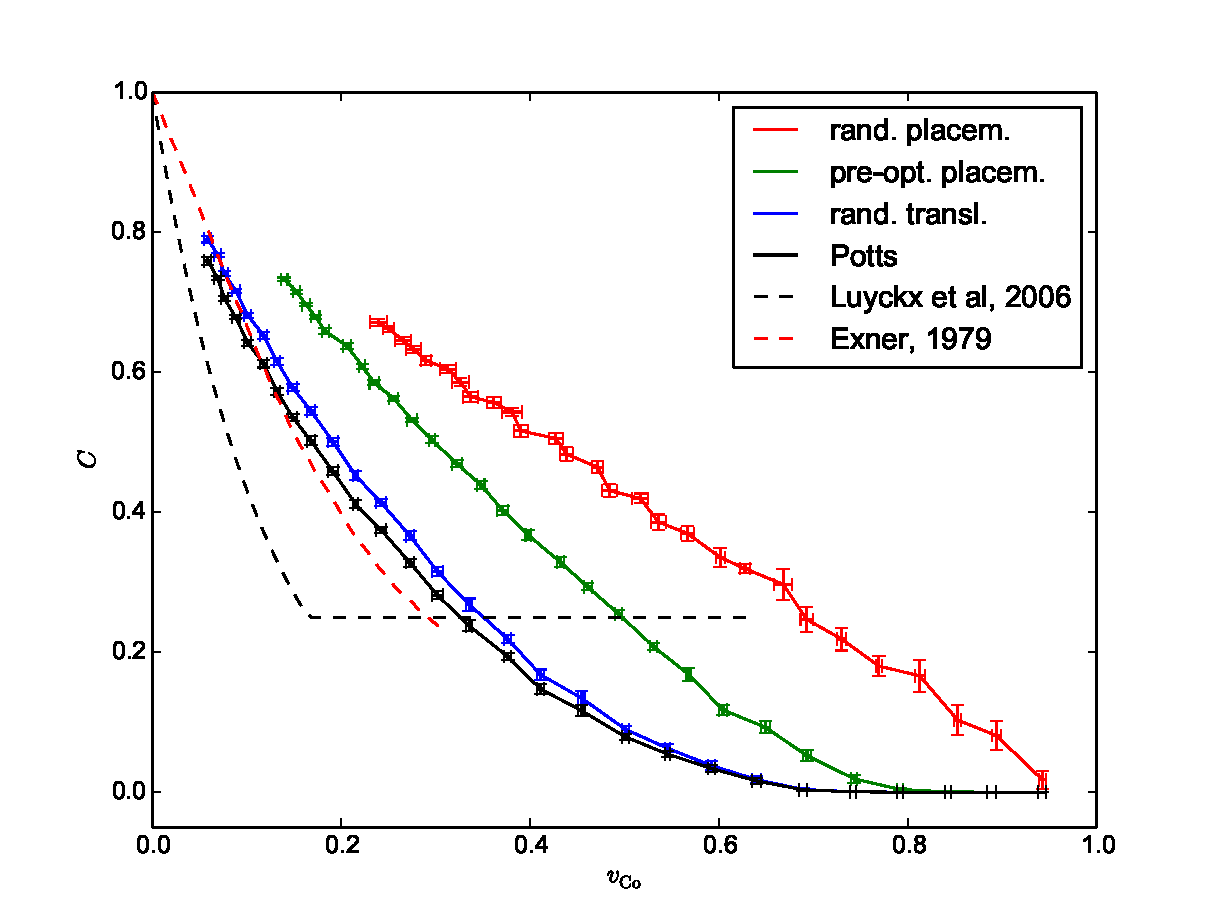
\includegraphics[width=0.6\linewidth]{Result_plots/runs1/contiguity}
  \caption{Sensitivity analysis for $m$. Bars indicate one standard deviation.}
  \label{fig:sens_m}
\end{figure}

Results for varying $m$ is given in Figure~\ref{fig:sens_m}.
The analysis was set up with 5 realizations with $L = \SI{10}{\micro\meter}$ and the target volume fraction $v_{\WC,\text{goal}} = 1.0$.
%and the Potts model simulation using $\text{MC}_\text{steps} = 10 M^3$.
The primary reason for the lowered contiguity is that the increased resolution allows for thinner wedges of Co between grains, effectively increasing the phase boundary area, thus lowering the contiguity.
For complete convergence, the study indicates that the resolution should be set quite high, possibly $m \geq 30$, to fully capture the thinnest Co layers.
The overall grain structure is however captured well even at lower resolutions, $m \approx $ 10--20.

The packing using random translations works well even with a coarse, and $m_\text{coarse} = 8 L$ is a good trade-off between accuracy and performance.
This coarse grid should only be used to obtain coordinates of the grains in the packing stage, as the final grid resolution should be higher to better resolve the grain geometry.


\subsection{Sensitivity to window size}
%%%%%%%%%%%%%%%%%%%%%%%%%%%%%%%%%%%%%%%%%%%%%%%%
%%%%%%%%%%%%%%%%%%%%%%%%%%%%%%%%%%%%%%%%%%%%%%%% L
%%%%%%%%%%%%%%%%%%%%%%%%%%%%%%%%%%%%%%%%%%%%%%%%
\begin{figure}[H]
  \centering

  \begin{tikzpicture}[font=\footnotesize]
  \begin{axis}[
%       xmax = 1,
%       xmin = 0.,
      ymin = 0.43,
      %ymax = 0.59,
      legend pos=south east,
      legend style={font=\tiny},
      legend style={draw=none},
      xlabel={$L$ [\si{\micro\meter}]},
      ylabel={$C$},
      width=0.45\linewidth
      ]

    \addplot[red, error bars/.cd, y dir=both, y explicit]
	table[x=L, y=cont_mean, y error expr=\thisrow{cont_potts_std}] {stat_l_random.txt};
    \addlegendentry{Random placement}

    \addplot[green!50!black, error bars/.cd, y dir=both, y explicit]
	table[x=L, y=cont_mean, y error expr=\thisrow{cont_potts_std}] {stat_l_U.txt};
    \addlegendentry{Repulsive potential}
    
    \addplot[blue, error bars/.cd, y dir=both, y explicit]
	table[x=L, y=cont_mean, y error expr=\thisrow{cont_potts_std}] {stat_l_transl.txt};
    \addlegendentry{Random translations}
    
    
    \addplot[red, dashed, error bars/.cd, y dir=both, y explicit]
	table[x=L, y=cont_potts_mean, y error expr=\thisrow{cont_potts_std}] {stat_l_random.txt};
%     \addlegendentry{Random placement}

    \addplot[green!50!black, dashed, error bars/.cd, y dir=both, y explicit]
	table[x=L, y=cont_potts_mean, y error expr=\thisrow{cont_potts_std}] {stat_l_U.txt};
%     \addlegendentry{Repulsive potential}
    
    \addplot[blue, dashed, error bars/.cd, y dir=both, y explicit]
	table[x=L, y=cont_potts_mean, y error expr=\thisrow{cont_potts_std}] {stat_l_transl.txt};
%     \addlegendentry{Random translations}
  \end{axis}
  \end{tikzpicture}
  %
  \begin{tikzpicture}[font=\footnotesize]
  \begin{axis}[
%       xmax = 2.0,
%       xmin = 0.,
      ymin = 0.6,
      ymax = 0.9,
%       legend pos=south east,
      legend style={at={(0.95,0.5)}},
      legend style={font=\tiny},
      legend style={draw=none},
      xlabel={$L$ [\si{\micro\meter}]},
      ylabel={$v_\WC$},
      width=0.45\linewidth
      ]

    \addplot[red, error bars/.cd, y dir=both, y explicit]
	table[x=L, y expr=1-\thisrow{co_fracs_mean}, y error expr=\thisrow{co_fracs_std}] {stat_l_random.txt};
    \addlegendentry{Random placement}

    \addplot[green!50!black, error bars/.cd, y dir=both, y explicit]
	table[x=L, y expr=1-\thisrow{co_fracs_mean}, y error expr=\thisrow{co_fracs_std}] {stat_l_U.txt};
    \addlegendentry{Repulsive potential}
    
    \addplot[blue, error bars/.cd, y dir=both, y explicit]
	table[x=L, y expr=1-\thisrow{co_fracs_mean}, y error expr=\thisrow{co_fracs_std}] {stat_l_transl.txt};
    \addlegendentry{Random translations}
  \end{axis}
  \end{tikzpicture}
  %
  \begin{tikzpicture}[font=\footnotesize]
  \begin{axis}[
%       xmax = 1,
%       xmin = 0.,
      %ymin = 0.8,
%       ymax = 1.0,
%       legend pos=south east,
      legend style={at={(0.95,0.5)}},
      legend style={font=\tiny},
      legend style={draw=none},
      xlabel={$L$ [\si{\micro\meter}]},
      ylabel={$\mathop{\text{mean}}(d_{\text{eq}})$},
      width=0.45\linewidth
      ]

    \addplot[red, error bars/.cd, y dir=both, y explicit]
	table[x=L, y=d_eq_mean_mean, y error expr=\thisrow{d_eq_mean_std}] {stat_l_random.txt};
    \addlegendentry{Random placement}

    \addplot[green!50!black, error bars/.cd, y dir=both, y explicit]
	table[x=L, y=d_eq_mean_mean, y error expr=\thisrow{d_eq_mean_std}] {stat_l_U.txt};
    \addlegendentry{Repulsive potential}
    
    \addplot[blue, mark=-, error bars/.cd, y dir=both, y explicit]
	table[x=L, y=d_eq_mean_mean, y error expr=\thisrow{d_eq_mean_std}] {stat_l_transl.txt};
    \addlegendentry{Random translations}
  \end{axis}
  \end{tikzpicture}
  \caption{Sensitivity analysis for $L$. Bars indicate one standard deviation.}
  \label{fig:sens_L}
\end{figure}

Figure~\ref{fig:sens_L} show averages from 5 realizations using $m = 10$ and $v_{\WC,\text{goal}} = 1.0$.
%%%%%%%%%%%%% $\text{MC}_\text{steps} = 10 M^3$
The use of periodic boundary conditions should eliminate most of the boundary effects, and this is confirmed by the flat trends seen in Figure~\ref{fig:sens_L}.
Naturally, smaller windows will have a larger spread, particularly noticeable in the grain size distribution.


\subsection{Sensitivity to Monte-Carlo steps}

%%%%%%%%%%%%%%%%%%%%%%%%%%%%%%%%%%%%%%%%%%%%%%%%
%%%%%%%%%%%%%%%%%%%%%%%%%%%%%%%%%%%%%%%%%%%%%%%% MC_steps
%%%%%%%%%%%%%%%%%%%%%%%%%%%%%%%%%%%%%%%%%%%%%%%%
\begin{figure}[H]
  \centering

  \begin{tikzpicture}[font=\footnotesize]
  \begin{axis}[
%       xmax = 1,
%       xmin = 0.,
%       ymin = 0.45,
%       ymax = 0.6,
      xtick={0, 0.05, 0.1},
      legend pos=north east,
      legend style={font=\tiny},
      legend style={draw=none},
      xlabel={$\text{MC}_\text{steps}/M^4$},
      ylabel={$C$},
      width=0.45\linewidth
      ]

    \addplot[red]
	table[x=mc_steps, y=contiguity] {stat_mc_steps_random_10_L10.0.txt};
    \addlegendentry{Random placement $m =10$}

    \addplot[green!50!black]
	table[x=mc_steps, y=contiguity] {stat_mc_steps_U_10_L10.0.txt};
    \addlegendentry{Repulsive potential $m=10$}
    
    \addplot[blue]
	table[x=mc_steps, y=contiguity] {stat_mc_steps_transl_10_L10.0.txt};
    \addlegendentry{Random translations $m=10$}

    \end{axis}
  \end{tikzpicture}
  %
  \begin{tikzpicture}[font=\footnotesize]
  \begin{axis}[
%       xmax = 1,
%       xmin = 0.,
%       ymin = 0.45,
%       ymax = 0.6,
      xtick={0, 0.05, 0.1},
      legend pos=north east,
      legend style={font=\tiny},
      legend style={draw=none},
      xlabel={$\text{MC}_\text{steps}/M^4$},
      ylabel={$C$},
      width=0.45\linewidth
      ]

    \addplot[red]
	table[x=mc_steps, y=contiguity] {stat_mc_steps_random_20_L10.0.txt};
    \addlegendentry{Random placement $m=20$}

    \addplot[green!50!black]
	table[x=mc_steps, y=contiguity] {stat_mc_steps_U_20_L10.0.txt};
    \addlegendentry{Repulsive potential $m=20$}
    
    \addplot[blue]
	table[x=mc_steps, y=contiguity] {stat_mc_steps_transl_20_L10.0.txt};
    \addlegendentry{Random translations $m=20$}

    \end{axis}
  \end{tikzpicture}

  \caption{Convergence analysis for $\text{MC}_\text{steps}$}
  \label{fig:sens_MC_steps}
\end{figure}

A convergence analysis for $\text{MC}_\text{steps}$ is shown in Figure~\ref{fig:sens_MC_steps}, which was done on a a single realization using $L = \SI{10}{\micro\meter}$, $v_{\WC,\text{goal}} = 1.0$.
To speed up the simulation, the multigrid optimization described in Section~\ref{sec:strategy} is used.
The number of necessary Monte-Carlo steps should scale with $M^4$, two grid resolutions are tested.
%
% The Potts model simulation was done using the multi-grid optimization.
% It must be noted that more iterations are not necessarily better in this case, as the goal is to simulate real the material and not a strict minimization of areas.
%
The results show that using $\text{MC}_\text{steps} = 0.05 M^4$ is sufficient.



\subsection{Case-study}


\begin{figure}[htbp!]
 \centering
%  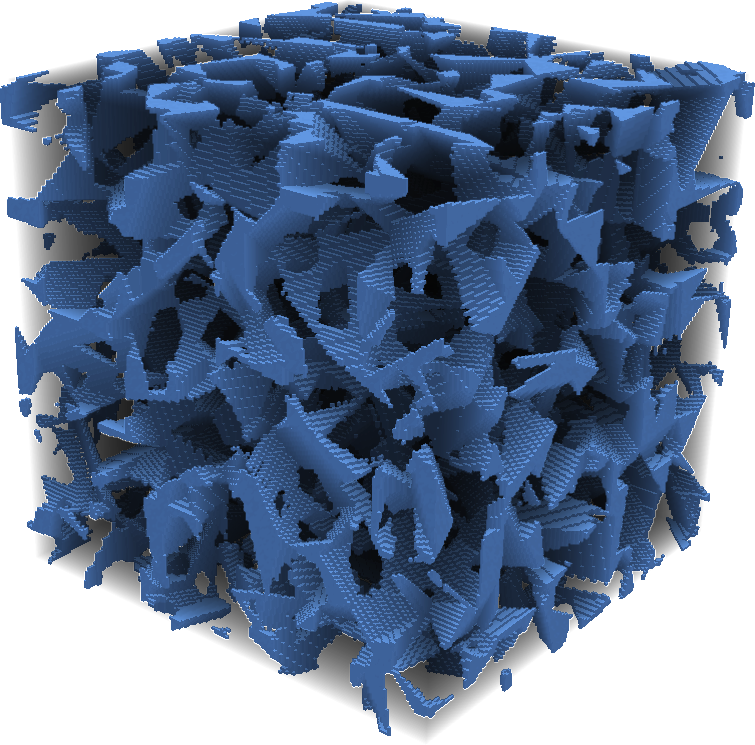
\includegraphics[width=0.48\linewidth]{co_matrix}
 %\includegraphics[width=0.5\linewidth]{ccbuilder_L10}
 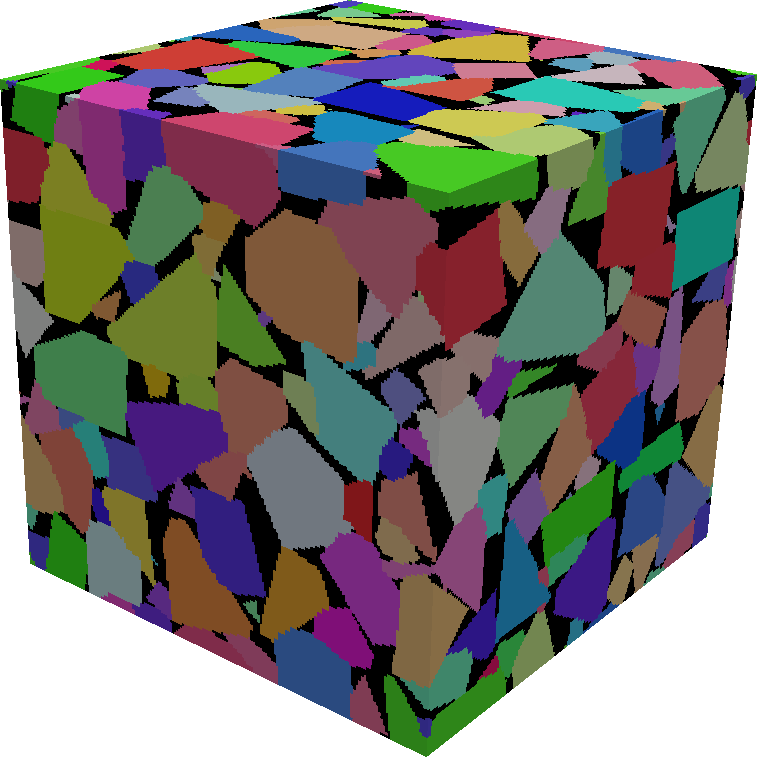
\includegraphics[width=0.5\linewidth]{WC_IPF.pdf}
 \caption{Example of CCBuilder output for with WC grains colored by IPF-colors with Co-matrix in black} \label{fig:final_example}
\end{figure}

\begin{figure}[htbp!]
 \centering
 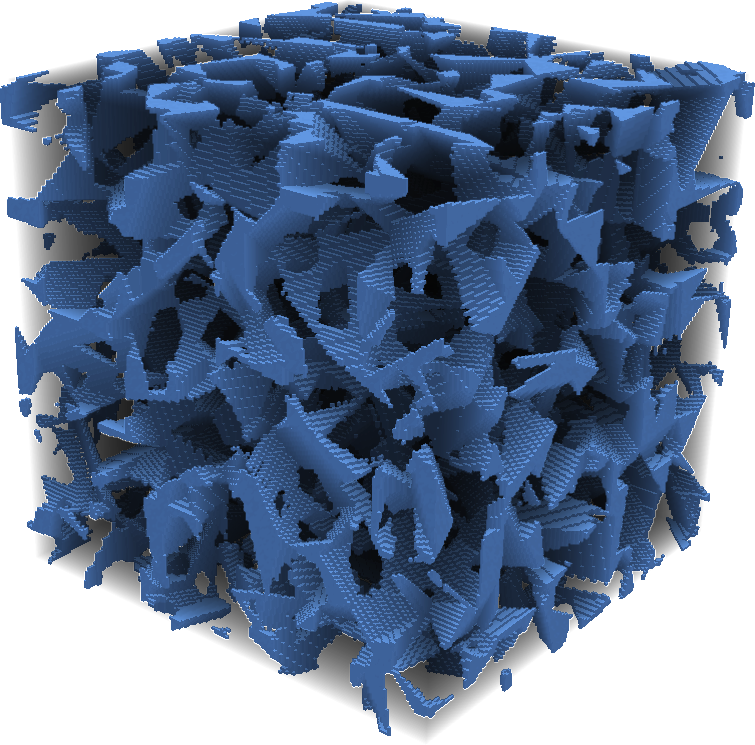
\includegraphics[width=0.5\linewidth]{co_matrix}
 \caption{Connected Co-matrix of a system with WC-grains hidden} \label{fig:final_example_co}
\end{figure}


% 
% \begin{figure}[H]
%  \centering
%  \includegraphics[width=0.3\linewidth]{voxel_rounding_errors}
%  \caption{Snapshot of Co-phase (transparent WC-phase) where voxel discretization errors generating unconnected Co-voxels when the thickness approaches the voxel size \label{fig:discretization_error}}
% \end{figure}

We will have a closer look at a generated microstructure using $d_\text{eq} \in U[0.5, 1.5]$, $k \in U[0.4, 1.4]$, $r \in U[0.1, 0.4]$, with the target volume fraction is set $v_{\WC,\text{goal}} = 1.0$. CCBuilder was set up using $m = 20$, packing using random translations with $\Delta = L/2$ and $NR_\text{tries}$, and Potts model simulation using $\text{MC}_\text{steps} = 0.1 M^4$.
The resulting output for $L = \SI{8}{\micro\meter}$ is illustrated in Figure~\ref{fig:final_example} and \ref{fig:final_example_co} with a volume fraction $v_\Co = 0.135$ and a contiguity of $C = 0.516$.

In real WC-Co microstructures, one finds that the Co FCC-lattice orientation is the same over large regions.
This indicates that the Co-matrix consists of large continuous grains.
The continuous and penetrating Co-matrix is an important aspect in the manufacturing process.
To verify this property in CCBuilder the function \verb+compute_co_grain_sizes+ labels all isolated regions of Co with respect to the periodic boundary conditions.
Experimentally it is found that the Co-matrix is continuous even at high volume fraction WC, $v_\WC = 0.95$, and this important property is also preserved in CCBuilder.
If this property is important for further analysis, it is important to use a very fine grid, e.g. $m \geq 40$, in order to minimize the discretization errors.
These discretization errors are more frequent for high $v_\WC$, as slivers of Co is often created during the packing stage.
In all simulations, the Co phase has been a continuous interpenetrating network, with some small isolated pockets of Co present.


%%%%%%%%%%%%%%%%%%%%%%%%%%%%%%%%%%%%%%%%%%%%%%%%%%%%%%%%%%%%%%%%%%%%%%%%%%%%%%%%%%%%%%
%%%%%%%%%%%%%%%%%%%%%%%%%%%%%%%%%%%%%%%%%%%%%%%%%%%%%%%%%%%%%%%%%%%%%%%%%%%%%%%%%%%%%%
%%%%%%%%%%%%%%%%%%%%%%%%%%%%%%%%%%%%%%%%%%%%%%%%%%%%%%%%%%%%%%%%%%%%%%%%%%%%%%%%%%%%%%
\subsubsection{Grain size distribution}
\label{sec:grain_size_dist}


\begin{figure}[htbp!]
\centering
 \begin{tikzpicture}[font=\footnotesize]
 \begin{axis}[
      %xmin=0, xmax=2,
      legend style={draw=none},
      legend pos=outer north east,
      xlabel={$d_\text{eq}$ [\si{\micro\meter}]},
      ylabel={Probability density}
      %height=5cm,
      %width=8cm
      ]
%   \addplot[fill=blue!20, draw=none, forget plot, hist={bins=20, density, data min=0, data max=104.4775}] table[y index=0]  {misorientation.txt};

    \addplot [fill=blue, blue, opacity=0.3, ultra thick, draw=none, ybar, bar width=11pt, raw gnuplot] gnuplot {
      binwidth=0.1;
      bin(x,bw)=bw*floor(x/bw)+bw/2;
      stats 'd_eq_orig.txt';
      plot 'd_eq_orig.txt' using (bin(column(1),binwidth)):(1./(binwidth * STATS_records)) smooth freq with boxes;
    };
    \addlegendentry{Initial}

    \addplot [fill=red, red, opacity=0.3, ultra thick, draw=none, ybar, bar width=11pt, raw gnuplot] gnuplot {
      binwidth=0.1;
      bin(x,bw)=bw*floor(x/bw)+bw/2;
      stats 'd_eq_2.txt';
      plot 'd_eq_2.txt' using (bin(column(1),binwidth)):(1./(binwidth * STATS_records)) smooth freq with boxes;
    };
    \addlegendentry{Final}
 \end{axis}
 \end{tikzpicture}
 \caption{Example of initial and final size distribution of WC grains.} \label{fig:grain_distribution}
\end{figure}

In Figure~\ref{fig:grain_distribution} we show the full grain size distribution before insertion and after insertion, for $L = \SI{20}{\micro\meter}$, $m = 10$, $v_{\WC,\text{goal}} = 1.00$, producing $12118$ WC grains.
Values are initially generated from a uniform distribution, $d_\text{eq} \in U[0.5, 1.5]\,\si{\micro\meter}$ and the repulsive potential is used for a high packing factor..
The final distribution is skewed towards the lower values, as is expected from the overlap.
% Unfortunately, the grain size (and shape) distributions are rarely documented, leaving the contiguity as the only experimental target in this paper.
% CCBuilder supports the option to plug in any predefined distributions for the grain parameters $k$, $r$, or $d_\text{eq}$.
To replicate an experimental distribution, a clever choice of initial distribution must be made.
% {\color{red} PROBLEM: I can't list MC iterations because the parameter has changed meaning in the new code now... they are just ``enough'' to converge.}



%%%%%%%%%%%%%%%%%%%%%%%%%%%%%%%%%%%%%%%%%%%%%%%%%%%%%%%%%%%%%%%%%%%%%%%%%%%%%%%%%%%%%%
%%%%%%%%%%%%%%%%%%%%%%%%%%%%%%%%%%%%%%%%%%%%%%%%%%%%%%%%%%%%%%%%%%%%%%%%%%%%%%%%%%%%%%
%%%%%%%%%%%%%%%%%%%%%%%%%%%%%%%%%%%%%%%%%%%%%%%%%%%%%%%%%%%%%%%%%%%%%%%%%%%%%%%%%%%%%%
\subsubsection{Misorientation}
Misorientation is the measure of the angle between contacting crystals lattices.
This is measured to ensure that the packing strategy doesn't have and unwanted influences due to grain geometry.
Trigonal crystallographic symmetries are used when computing the misorientation.
Neighboring grains are identified at voxel level, and the misorientation is computed for each contacting grain pair.

\begin{figure}[htbp!]
\centering
 \begin{tikzpicture}[font=\footnotesize]
 \begin{axis}[
      xmin=0, xmax=104.4775,
      legend style={draw=none},
      legend pos=north west,
      %ylabel style={font=\Huge}
      xticklabels={0, 0$^{\circ}$ , 20$^{\circ}$, 40$^{\circ}$, 60$^{\circ}$, 80$^{\circ}$, 100$^{\circ}$},
      xlabel={Misorientation},% [${}^{\circ}$]}
      ylabel={Probability density},
      height=5cm,
      width=8cm
      ]
%   \addplot[fill=blue!20, draw=none, forget plot, hist={bins=20, density, data min=0, data max=104.4775}] table[y index=0]  {misorientation.txt};

    \addplot [fill=blue, blue, opacity=0.3, ultra thick, draw=none, ybar, bar width=9pt, raw gnuplot] gnuplot {
      binwidth=5;
      bin(x,bw)=bw*floor(x/bw)+bw/2;
      stats 'misorientation.txt';
      plot 'misorientation.txt' using (bin(column(1),binwidth)):(1./(binwidth * STATS_records)) smooth freq with boxes;
    };
  \addlegendentry{Generated}
  \addplot[densely dashed] table{D3.txt};
  \addlegendentry{Theoretical}
 \end{axis}
 \end{tikzpicture}
 \caption{Generated and theoretical misorientation angle distribution for trigonal symmetry} \label{fig:misorientation_large}
\end{figure}


Figure \ref{fig:misorientation_large} show the misorientation distribution for a large microstructure containing 5677 grains with good agreement with the theoretical distribution from \cite{morawiec_orientations_2004} for grains with random orientation.
These results verify numerically that the placement strategy for the grains are not inducing unwanted macroscopic anisotropy.
With the frequent $\Sigma$2 boundaries as seen in Figure \ref{fig:sigma_2}, one should expect a peaks at \SI{90}{\degree}, however, these are currently not included in CCBuilder.



\subsection{Effect of grain shape and size distribution on packing strategy}

\begin{figure}[H]
  \centering

  \begin{tikzpicture}[font=\footnotesize]
  \begin{axis}[
      xmax = 1,
      xmin = 0.,
      ymin = 0.0,
      ymax = 1.0,
      legend pos=outer north east,
      legend style={font=\tiny},
      legend style={draw=none},
      xlabel={$v_\Co$},
      ylabel={$C$},
      width=0.45\linewidth
      ]
    \addplot[gray, mark=x, only marks,forget plot] table[x index=8,y index=3]  {luyckx_table.txt};
%     \addlegendentry{Ultra fine}
    \addplot[gray, mark=x, only marks,forget plot] table[x index=8,y index=7]  {luyckx_table.txt};
%     \addlegendentry{Fine}
    \addplot[gray, mark=x, only marks,forget plot] table[x index=8,y index=12]  {luyckx_table.txt};
%     \addlegendentry{Medium}
    \addplot[gray, mark=x, only marks] table[x index=8,y index=16]  {luyckx_table.txt};
%     \addlegendentry{Coarse}
    \addlegendentry{Luyckx et al.\ (2006)}
    \addplot[gray, mark=*, only marks] coordinates { (0.15, 0.42) };
    \addlegendentry{Chang et al.\ (2015)}
    \addplot[gray,mark=square, only marks] table[x index=0,y index=1]  {exner_direct_data.txt};
    \addlegendentry{Exner (1966)}
    
    \addplot[green!50!black, solid]
	table[x=co_fracs_mean, y=cont_potts_mean] {stat_vol_U_L10.0.txt};
    \addlegendentry{Repulsive pot. uniform}
    
    \addplot[blue, solid]
	table[x=co_fracs_mean, y=cont_potts_mean] {stat_vol_transl_L10.0.txt};
    \addlegendentry{Random transl. uniform }


    \addplot[green!50!black, dashed]
	table[x=co_fracs_mean, y=cont_potts_mean] {stat_vol_U_const_L10.0.txt};
    \addlegendentry{Repulsive pot. constant}
    
    \addplot[blue, dashed]
	table[x=co_fracs_mean, y=cont_potts_mean] {stat_vol_transl_const_L10.0.txt};
    \addlegendentry{Random transl. constant}


%     \addplot[green!50!black, dashed]
% 	table[x=co_fracs_mean, y=cont_potts_mean] {stat_vol_U_u2_L10.0.txt};
%     \addlegendentry{Repulsive pot. uniform 2}
%     
%     \addplot[blue, dashed]
% 	table[x=co_fracs_mean, y=cont_potts_mean] {stat_vol_transl_u2_L10.0.txt};
%     \addlegendentry{Random transl. uniform 2}
   
        
%     \addplot[green!50!black, dotted]
% 	table[x=co_fracs_mean, y=cont_potts_mean] {stat_vol_U_weibull_L10.0.txt};
%     \addlegendentry{Repulsive pot. Weibull}
%     
%     \addplot[blue, dotted]
% 	table[x=co_fracs_mean, y=cont_potts_mean] {stat_vol_transl_weibull_L10.0.txt};
%     \addlegendentry{Random transl. Weibull}

  \end{axis}
  \end{tikzpicture}
  \caption{Average contiguity ($C$) for different grain size ($d_\text{eq}$) distributions}
  \label{fig:deq_compare}
\end{figure}

In Figure~\ref{fig:deq_compare} we investigate the how the grain size distribution effects the final results in the two packing strategies.
The solid lines show $d_\text{eq} \in U[0.5, 1.5]\, \si{\micro\meter}$ and the dashed lines show the extreme case of a constant grain size $d_\text{eq} = \SI{1}{\micro\meter}$.
The simulations are run using $m = 10$, $L = \SI{10}{\micro\meter}$ and $\text{MC}_\text{steps} = 0.1 M^4$.
The repulsive potential gives similar results for both cases while the random translations show a significant loss in packing factor, and thus increases the contiguity significantly.



\begin{figure}[H]
  \centering

  \begin{tikzpicture}[font=\footnotesize]
  \begin{axis}[
      xmax = 1,
      xmin = 0.,
      ymin = 0.0,
      ymax = 1.0,
      legend pos=outer north east,
      legend style={font=\tiny},
      legend style={draw=none},
      xlabel={$v_\Co$},
      ylabel={$C$},
      width=0.45\linewidth
      ]
    \addplot[gray, mark=x, only marks,forget plot] table[x index=8,y index=3]  {luyckx_table.txt};
%     \addlegendentry{Ultra fine}
    \addplot[gray, mark=x, only marks,forget plot] table[x index=8,y index=7]  {luyckx_table.txt};
%     \addlegendentry{Fine}
    \addplot[gray, mark=x, only marks,forget plot] table[x index=8,y index=12]  {luyckx_table.txt};
%     \addlegendentry{Medium}
    \addplot[gray, mark=x, only marks] table[x index=8,y index=16]  {luyckx_table.txt};
%     \addlegendentry{Coarse}
    \addlegendentry{Luyckx et al.\ (2006)}
    \addplot[gray, mark=*, only marks] coordinates { (0.15, 0.42) };
    \addlegendentry{Chang et al.\ (2015)}
    \addplot[gray,mark=square, only marks] table[x index=0,y index=1]  {exner_direct_data.txt};
    \addlegendentry{Exner (1966)}

    \addplot[green!50!black, solid]
	table[x=co_fracs_mean, y=cont_potts_mean] {stat_vol_U_L10.0.txt};
    \addlegendentry{Repulsive pot. high $k$}
    
    \addplot[blue, solid]
	table[x=co_fracs_mean, y=cont_potts_mean] {stat_vol_transl_L10.0.txt};
    \addlegendentry{Random transl. high $k$}

    \addplot[green!50!black, dashed]
	table[x=co_fracs_mean, y=cont_potts_mean] {stat_vol_U_lowk_L10.0.txt};
    \addlegendentry{Repulsive pot. low $k$}
    
    \addplot[blue, dashed]
	table[x=co_fracs_mean, y=cont_potts_mean] {stat_vol_transl_lowk_L10.0.txt};
    \addlegendentry{Random transl. low $k$}
    
  \end{axis}
  \end{tikzpicture}
  \caption{Results of different grain shape ($k$) distributions compared with experimental data}
  \label{fig:k_compare}
\end{figure}

Different distributions of $k$ are also investigated in Figure~\ref{fig:k_compare}; solid lines show $U[0.1, 0.4]$ and dashed lines show $U[0.4, 1.4]$.
These values correspond to WC-Co systems with high $W$ or high $C$ content respectively \cite{lay_morphology_2008}.
The higher $k$ leads to a grain shape that is much closer to the approximated spherical shape used in the repulsive potential, drastically increasing the packing factor.


We can obtain excellent agreement with Exners data \cite{exner_physical_1979} using the random translation packing method.
The data from Luyckx et al.\ \cite{luyckx_dependence_2006} shows very low contiguities at $v_\Co < 0.2$, and a new approach is likely required in order to reproduce this in CCBuilder.
%
%
Inclusion of $\Sigma$2 boundaries would increase the contiguity, especially at higher $v_\Co$ levels.
This trend can be seen in Luyckx's data in Figure~\ref{fig:deq_compare}, \ref{fig:k_compare}.
However, CCBuilder is designed for $v_\Co$ in the 5--30\%\ range, as this is the range found in industrial hardmetals.


%%%%%%%%%%%%%%%%%%%%%%%%%%%%%%%%%%%%%%%%%%%%%%%%%%%%%%%%%%%%%%%%%%%%%%%%%%%%%%%%%%%%%%%%%%%%%%%%%%%
%%%%%%%%%%%%%%%%%%%%%%%%%%%%%%%%%%%%%%%%%%%%%%%%%%%%%%%%%%%%%%%%%%%%%%%%%%%%%%%%%%%%%%%%%%%%%%%%%%%
%%%%%%%%%%%%%%%%%%%%%%%%%%%%%%%%%%%%%%%%%%%%%%%%%%%%%%%%%%%%%%%%%%%%%%%%%%%%%%%%%%%%%%%%%%%%%%%%%%%
\section{Conclusions and outlook}

The generated microstructure closely matches the real WC-Co microstructure both visually and in terms of the important statistical measurements.
Currently missing is the common $\Sigma$2 boundaries that occur inside grains (causing the crystal structure to realign inside the grain).
This could be achieved by constructing grains consisting of several sub-grains connected by $\Sigma$2 intra-grain boundaries.

Compensating for the overlap when targeting a final volume fraction $v_\WC$ is straight forward using \eqref{eq:inverse_v_wc}, but in order to replicate experimental grain size distributions, more work is needed to find suitable heuristics for the initial size distributions.

% At the lowest volume fraction though this difference could possible be due to a flawed initial grain size distribution.
% Larger grain size variations would lead to lowered contiguity of the carbide phase.

The Potts model simulation is currently assuming isotropic surface energy, and minimizes inter-grain surfaces.
This simulation could be improved by taking into account the misorientation between the WC grains.
The method for computing the grain boundary area is only based on the 6 directly neighboring voxels, which is a poor approximation of the real boundaries at anything but 90 degree angles.
Improved methods for approximating grain boundary areas could be implemented by computing local curvatures, though the possibility of multiple neighboring grains and phases adds complexity to the implementation.
In addition, the value of $\tau$ was not found to have any noticeable effect.

With the computational time scaling with $M^3$, the multigrid optimizations techniques are vital for performance.
Using these techniques, the simulation time down of moderate sized problems ($L = 10\si{\micro\meter}$, $m = 20$) is below 2 minutes.
The control script included with CCBuilder comes predefined with the best known setup of parameters.

While CCBuilder is capable of directly exporting data for finite element analysis, the finite element mesh is tied to the resolution of the voxel grid.
Through surface reconstruction one could both lower the computational costs and open up the possibility to model inter-grain sliding.
Development of this extension is currently under progress.

Even with the present limitations, the realism is still high in the generated microstructures.
In addition to the statistical properties, the generated microstructure in Figure~\ref{fig:potts_before_after} is visually very similar to the micrograph in Figure~\ref{fig:wc-co_hardmetal}, both with the same volume fraction Co.
The results are fully useable for state of the art finite element analysis on key engineering properties of WC-Co hardmetals, with high predictive capabilities.

%\printbibliography

\bibliographystyle{elsarticle-num}
\bibliography{Sintering,Multiscale}

\end{document}
